\documentclass{csnotes_eng}

% ==============================================================================
% DOCUMENT SPECIFIC CUSTOMIZATIONS
% ==============================================================================

% --------------------------- START CUSTOMIZATIONS -----------------------------

% You can add any custom packages or commands specific to this document here

\usepackage{array}
\usepackage{booktabs}
\usetikzlibrary{shapes, arrows, positioning}

\newcommand{\Path}[1]{\operatorname{path}\left(#1 \right)}
\newcommand{\Reversed}[1]{\operatorname{reversed}\left(#1\right)}

\setabstracttitle{Purpose of the Document}

\newcommand{\whitepage}{
  \newpage
  \thispagestyle{empty}
  \mbox{}
  \newpage
}

% ---------------------------- END CUSTOMIZATIONS ------------------------------

% ==============================================================================
% DOCUMENT INFORMATION
% ==============================================================================
\title{NoSQL Databases}
\author{Riccardo Regina}
\date{\today}

% Additional information for the title page
\university{University of Naples Federico II}
\department{Department of Electrical Engineering and Information Technology}
\course{Master's Degree in Computer Science}
\subject{NoSQL Databases}
\academicyear{Academic Year 2025/2026}

% ==============================================================================
% BIBLIOGRAPHY
% ==============================================================================
% Specify the .bib file with your bibliographic references
% Uncomment the following line when you have created the bibliography.bib file
\addbibresource{bibliography.bib}

% ==============================================================================
% INIZIO DOCUMENTO
% ==============================================================================

\begin{document}

\pagenumbering{gobble}

\maketitlepage{}

\whitepage{}

\newgeometry{top=2cm}
\tableofcontents
\restoregeometry{}

\whitepage{}

\pagenumbering{arabic}
\setcounter{page}{1}

\begin{abstract}
  This document contains notes and study materials related to the \textit{Advanced Databases: NoSQL} course taught by Prof.~A.~Calì at the University of Naples Federico II during the academic year 2025/26.

  \textbf{These notes are intended to support students in their learning journey and provide a reference resource for the topics discussed during the course. However, they do not replace the official materials or the instructor's lectures in any way.}
  This document is created by students, for students, and may therefore contain errors or inaccuracies.

  On this subject, the document will include some content not directly sourced from the lessons, but added or modified by the authors to improve the clarity or depth of the topics covered.

  We commit to verifying any substantial changes to the original material with the instructor. However, if such verification has not yet taken place, indicators will be included to signal any deviations from the official material. Specifically:

  \begin{itemize}
      \item Content added or substantially modified by the authors will be marked with the symbol \warningsymbol{};
      \item Content that has undergone only structural or formatting reorganization will be marked with the symbol \infosymbol{};
      \item Any additional content not presented in the lessons but verified with the instructor will be marked with the symbol \extrasymbol{}.
  \end{itemize}

  \begin{flushright}
    \vspace{2cm}
    \textbf{The author:}\\
    \href{https://github.com/riccardoregina}{Riccardo Regina} \\
  \end{flushright}
\end{abstract}
\chapter{The Rise of NoSQL}
For a large part of software history, relational databases have been the only adopted DBMS paradigm. Over the years, several alternatives were proposed --- such as deductive databases, object-oriented databases, and XML databases --- but none achieved lasting commercial success. A persistent issue with relational databases is the \keyword{impedance mismatch}: the structural and philosophical difference between the relational model (based on tables, rows, and set-oriented operations) and the object-oriented programming model (based on classes, objects, and references)\cite{sadalage2012nosql}. This mismatch forces developers to write complex translation logic between the application's in-memory object graph and the database's flat relational representation.

Object-oriented databases attempted to solve this problem natively, but they swiftly faded into oblivion due to various shortcomings, including the lack of a solid theoretical foundation comparable to the relational model and poor integration with existing tools. In their place, \textbf{Object-Relational Mappers (ORMs)} became widespread, automating much of the mapping code while still operating over a relational backend. To gain further decoupling from the specific DBMS and to serve data over the web more naturally, the industry increasingly adopted \keyword{Application Databases} --- databases that serve data directly through an HTTP API, often backed by a relational store but hidden behind a service layer.

Another critical limitation of relational databases is that they were primarily designed for single-server deployments and \textbf{do not scale well on clusters} (distributed environments), particularly when consistency and availability are required simultaneously across many nodes\cite{kleppmann2017ddia}. \keyword{NoSQL} databases emerged to address these challenges: they are generally non-relational by design and are built from the ground up to run efficiently on large clusters.

\section{Data Models and Storage Models}
A \keyword{data model} is a set of constructs and rules used to represent and organize information within a database. It defines how data are structured and manipulated. A \keyword{storage model}, on the other hand, describes how a DBMS physically stores, organizes, and retrieves data internally on the storage medium. The data model influences the logical view provided to the user, while the storage model determines performance characteristics such as read/write speed and memory footprint.

Among the data models adopted by NoSQL systems, two major families can be identified:
\begin{itemize}
    \item \textbf{Aggregate-oriented models}: Key-value, Document, and Column-family stores.
    \item \textbf{Graph-based models}: Designed for highly interconnected data.
\end{itemize}

\section{Aggregates}
The term \keyword{aggregate} originates from Domain-Driven Design (DDD)\cite{evans2003ddd}. A DDD aggregate is a cluster of domain objects that can be treated as a single unit. An example is an \emph{order} together with its \emph{line-items}: while they are separate objects, it is useful to treat the order and all its line items as a single aggregate\cite{fowler2013aggregate}.

Every aggregate has one of its component objects designated as the \keyword{aggregate root}. Any reference from outside the aggregate boundary should only point to the aggregate root, never to the internal objects. This allows the root to act as a gatekeeper, ensuring the integrity and enforcing the invariants of the aggregate as a whole. Aggregates are the basic unit of transfer for data storage: you request to load or save entire aggregates. Transactions should \textbf{not cross aggregate boundaries}; all changes within an aggregate are committed atomically, but changes spanning multiple aggregates must be handled with eventual consistency or compensating actions at the application level.

\begin{warning}{Not to be confused with collections}
    DDD aggregates should not be confused with generic collection classes (lists, maps, sets). DDD aggregates are domain-specific concepts --- an order, a clinic visit, a playlist --- while collections are generic data structures. An aggregate will often contain multiple collections together with simple fields. The term \q{aggregate} also appears in other contexts (e.g., UML class diagrams), where it denotes a different concept (a whole-part relationship) and does \emph{not} carry the DDD-specific semantics described here.
\end{warning}

Aggregates are the key to scaling well on clusters because they form a natural unit for:
\begin{itemize}
    \item \keyword{Replication}: The aggregate can be copied across multiple nodes to increase availability and read performance.
    \item \keyword{Sharding} (horizontal partitioning): Different aggregates can be distributed across different nodes based on a shard key, allowing the database to store data in a distributed manner.
\end{itemize}

\subsection{Transactions}
A \keyword{transaction} is a sequence of operations performed as a single logical unit of work. In relational databases, transactions are expected to satisfy the \keyword{ACID} properties:
\begin{itemize}
    \item \textbf{Atomicity}: All operations in the transaction complete successfully, or none do.
    \item \textbf{Consistency}: The transaction brings the database from one valid state to another.
    \item \textbf{Isolation}: Concurrent transactions do not interfere with each other.
    \item \textbf{Durability}: Once committed, the results persist even in the event of a failure.
\end{itemize}
Aggregate-oriented databases can typically guarantee ACID properties \textbf{within a single aggregate} but cannot do so across cross-aggregate operations, which must be handled at the application level or with eventual consistency.

\subsection{Relationships}
In aggregate-oriented databases, relationships between aggregates are typically handled through \keyword{value-based correspondence}: rather than using foreign keys and joins as in the relational model, one aggregate stores the identifier of another aggregate's root. 
This approach reflects the DDD principle that references between aggregates should only go through their roots.

Consequently, \textbf{joins are delegated to the application layer}. 
To reconstruct a relationship, the application must retrieve the first aggregate, extract the referenced identifier, and then issue a separate query to fetch the related aggregate. 
The database itself does not perform server-side joins across aggregate boundaries. 
This design trades immediate referential convenience for the ability to distribute aggregates independently across a cluster: delegating joins to the application allows each aggregate to be scaled independently, without being tied to the physical location of related aggregates.

That said, some NoSQL databases do make relationships visible to the DBMS. 
For instance, graph databases are natively relationship-oriented and allow efficient traversal of connections. 
Even some document databases (like MongoDB) offer \code{\$lookup} operators that simulate a left outer join between collections, though these are typically recommended for occasional use rather than as a replacement for proper aggregate design.

With respect to updates, the fundamental unit of data retrieval and persistence is the \textbf{aggregate itself}. When an application reads an aggregate, it receives a self-contained, complete snapshot of that domain unit --- not just a flat row that must be reassembled. This means:
\begin{itemize}
    \item The aggregate is the \textbf{atomic unit of writes}: all changes to the aggregate (including nested objects and collections) are saved together.
    \item The aggregate is the \textbf{natural unit of reads}: the application loads the entire aggregate in one operation, which aligns with how the data will be used in business logic.
    \item Because related aggregates are separate, updating multiple aggregates in response to a single business operation requires the application to coordinate the writes, often relying on eventual consistency patterns rather than distributed transactions.
\end{itemize}

\subsection{Materialized Views}
A \keyword{materialized view} is a pre-computed, persisted result of a query that is stored as a concrete data structure on disk. Unlike a standard (virtual) view in relational databases, which is merely a saved query that gets re-executed each time it is referenced, a materialized view holds the actual data resulting from that query. The DBMS keeps the materialized view up to date by recomputing it (or incrementally updating it) when the underlying base data changes.

In the context of NoSQL databases, materialized views serve several critical purposes:
\begin{itemize}
    \item \textbf{Supporting different query patterns}: In aggregate-oriented databases, data are modeled around a primary access pattern determined by the aggregate root. When an application needs to access the same data through a different aggregate boundary (e.g., querying orders by customer rather than by order ID), a materialized view can be built with the new access pattern as its primary key, effectively creating a pre-joined, query-optimized representation of the data.
    \item \textbf{Improving read performance}: By pre-computing expensive aggregations, joins, or transformations, materialized views eliminate the need to perform these operations at query time. This is especially valuable in distributed NoSQL systems where server-side joins are not available and application-level joins are prohibitively expensive.
    \item \textbf{Enabling real-time analytics}: Many NoSQL systems use materialized views to serve analytical queries without burdening the operational (OLTP) workload. The view can be updated asynchronously and queried independently.
\end{itemize}
The trade-off is that materialized views introduce \textbf{eventual consistency}: the data in the view may lag behind updates to the primary aggregates until the view is refreshed. The application must be designed to tolerate this delay. Prominent NoSQL databases that support materialized views include \textbf{Cassandra} (with its Materialized Views feature) and \textbf{Couchbase}, which uses materialized views and global secondary indexes to support flexible queries over its document store.

\section{Key-Value Databases}
A \keyword{key-value database} is the simplest NoSQL data model. It stores data as a collection of pairs $\langle key, value \rangle$, where the \code{key} is a unique identifier and the \code{value} is an opaque blob of data. The database does not inspect or interpret the structure of the value; it treats it as an atomic aggregate. This makes key-value stores a \textbf{strongly aggregate-oriented} model: the aggregate boundary is the entire value.

To access a value, the only available primitive is a lookup by key. There is no way to query based on the internal structure of the value without retrieving it entirely. A prominent example of a key-value database is \textbf{Redis}, which stores values as strings and offers a rich set of in-memory data structures and operations.

\section{Document Databases}
A \keyword{document database} is also strongly aggregate-oriented, but with a crucial difference from key-value stores: the internal structure of the stored document (typically JSON, BSON, or XML) is \textbf{visible to the DBMS}. The database can parse the hierarchical structure of the document, index its fields, and allow queries based on those fields.

To access a document, the primary method is still by its unique key, but secondary queries on document attributes are fully supported. The aggregate here is the document itself, which often embeds related sub-objects and lists. A widely used example of a document database is \textbf{MongoDB}.

\begin{note}{Key-value vs Document}
    The boundary between key-value and document databases is subtle. A key-value store treats the value as a black box; a document store understands and allows queries on the internal content of the value. This makes document databases more flexible for complex read patterns.
\end{note}

\section{Column-Family Stores}
A \keyword{column-family store} (or wide-column store) is an aggregate-oriented model organized as a \textbf{two-level map}. The first level maps a \code{row key} to an aggregate (a collection of columns); the second level maps, within that aggregate, \code{column keys} to \code{values}. Columns can be grouped into \textbf{column families} to organize related attributes together.

This model is still strongly aggregate-oriented: all columns belonging to the same row key are stored together on disk, forming the aggregate. A well-known example is \textbf{Cassandra}, which supports both \keyword{skinny rows} (a fixed, small number of columns per row, much like a relational table) and \keyword{wide rows} (a potentially very large and dynamically varying number of columns, up to billions, behaving essentially as a sorted map).

\section{Graph Databases}
A \keyword{graph database} is a DBMS designed to store, manage, and query highly interconnected data by representing entities as \textbf{nodes} and relationships between them as \textbf{edges}. Both nodes and edges can have associated properties, which are key-value pairs describing their attributes. This model is explicitly relationship-centric: connections are first-class citizens of the data model, not something reconstructed at query time through joins.

Graph databases excel in scenarios where the connections between entities are as important as the entities themselves, and where the application must traverse these connections efficiently. Typical use cases include:
\begin{itemize}
    \item \textbf{Social networks}: modeling users (nodes) and their friendships, follows, or interactions (edges).
    \item \textbf{Recommendation engines}: traversing relationships like "users who bought X also bought Y" or "friends who liked Z."
    \item \textbf{Knowledge graphs}: representing entities and their semantic relationships (e.g., "Socrates -- is\_a --> Philosopher -- born\_in --> Athens").
    \item \textbf{Fraud detection}: identifying suspicious patterns by traversing complex networks of transactions, accounts, and devices.
    \item \textbf{Route planning and network topology}: mapping physical or logical connections like roads, cables, or dependencies.
\end{itemize}
A prominent example of a graph database is \textbf{Neo4j}, which implements the labeled property graph model. In Neo4j, nodes are grouped by labels (e.g., \code{Person}, \code{City}), edges have a type that defines the nature of the relationship (e.g., \code{LIVES\_IN}, \code{KNOWS}), and both can store arbitrary properties. Neo4j provides its own declarative query language, \textbf{Cypher}, designed specifically for graph traversals and pattern matching.

\subsection{Queries}
Queries in a graph database are fundamentally based on \textbf{graph traversal and pattern matching}. Rather than joining tables through foreign key relationships, a graph query specifies a pattern of nodes and edges to match against the stored graph. The DBMS then locates paths through the graph that satisfy the pattern and returns the matched elements.

For example, a Cypher query to find friends of friends of a given user looks like:
\begin{verbatim}
MATCH (u:User {name: 'Alice'})-[:KNOWS]->(friend)-[:KNOWS]->(fof)
RETURN fof.name
\end{verbatim}
This query describes a pattern to match (Alice knows someone who knows someone else), and the database engine walks the graph edges to find all matching paths.

Graph databases are extremely efficient at graph traversals due to their storage and indexing strategies. A key technique is \textbf{index-free adjacency}: each node physically stores direct references (pointers) to its adjacent nodes and edges on disk. To traverse from one node to a neighboring node, the database follows an in-memory or on-disk pointer directly to the target node's storage location. This is an \(O(1)\) operation per hop, \textbf{independent of the total size of the dataset}. In contrast, a relational database would need to perform an index lookup (typically \(O(\log n)\) per join) for each relationship traversal, and the cost compounds with each additional level of depth, making deep traversals prohibitively expensive.

\textbf{Node insertions and deletions} in graph databases are also generally efficient. Inserting a new node involves allocating storage for the node's properties and establishing direct pointer references to its edges. Deleting a node requires removing the node and updating the adjacency pointers of all nodes that had edges to it. Because relationships are stored as physical pointers rather than matched through external indexes, these operations remain local to the affected nodes and their immediate neighbors. The cost is proportional to the node's degree (number of incident edges), not to the total graph size.

\subsection{The Difference with Aggregate-oriented Databases}
Graph databases and aggregate-oriented databases embody fundamentally different philosophies regarding data modeling, consistency, and distribution:

\begin{itemize}
    \item \textbf{Data model focus}: Aggregate-oriented databases are designed around the concept of the aggregate as a self-contained, bounded unit of data that is read and written atomically. Relationships between aggregates are denormalized (stored as foreign key references) and navigated at the application level. Graph databases, conversely, treat relationships as first-class entities that are stored and navigated natively within the database. The graph model does not require pre-defining aggregate boundaries; any node can be reached from any other node by traversing edges, without crossing an artificial aggregate frontier.

    \item \textbf{Deployment model}: Most aggregate-oriented databases (key-value, document, column-family) are \textbf{distributed by design}, built to run across large clusters of commodity hardware. They achieve horizontal scalability through sharding and replication, with aggregates serving as the natural unit of distribution. Graph databases, however, \textbf{typically run on a single server} (or a small replicated cluster for high availability, not horizontal scale). The reason is that graph traversals inherently cross multiple nodes and edges, and partitioning a highly connected graph across a cluster inevitably cuts many edges, requiring expensive network round-trips for each hop. Most graph databases are not horizontally scalable for write-heavy or deeply connected workloads; they rely on vertical scaling and, in some cases, replication for read scaling.

    \item \textbf{Consistency and transactions}: Because graph databases usually run on a single machine, they can offer \textbf{full ACID transactions} spanning many nodes and edges. A complex traversal that reads and modifies dozens of nodes and their relationships can be wrapped in a single atomic, isolated transaction. Aggregate-oriented databases, being distributed across many machines, typically guarantee ACID properties \textbf{only within a single aggregate} (on a single node). Cross-aggregate operations require the application to implement eventual consistency, compensating transactions, or distributed consensus protocols (which are slow and rarely used by default). This means that a graph database can natively support a use case like "transfer money from account A to account B while updating all related transaction records" atomically, whereas an aggregate-oriented database would require the application to break this into multiple writes and handle partial failures explicitly.
\end{itemize}

\subsection{Schema-less}
Like aggregate-oriented databases, most graph databases are \textbf{schema-less} by default. This means the database engine does not enforce a rigid, predefined structure on the data. Nodes and edges of the same type can have different properties, and new property types can be introduced at any time without altering a schema definition. In Neo4j, for instance, one \code{Person} node can have properties \code{\{name: "Alice", age: 30\}} while another \code{Person} node has \code{\{name: "Bob", city: "London"\}}; both are valid.

\begin{warning}{Schemaless \(\neq\) Without Schema}
    The term \q{schema-less} is potentially misleading. Every database that stores useful information has an \textbf{implicit schema} --- the set of conventions, property names, data types, and structural patterns that the application code and the users \emph{expect} the data to follow. Without any such expectations, querying becomes impossible (you cannot query \code{age > 25} if you do not know whether \code{age} exists or what type it holds). Schema-less simply means that the database does \emph{not validate or enforce} these expectations; the responsibility for maintaining a consistent logical structure is shifted entirely to the application layer.
\end{warning}

This shift brings both benefits and costs:
\begin{itemize}
    \item \textbf{Flexibility}: Developers can evolve the data model incrementally without costly schema migrations. New properties can be added to some nodes or edges while others remain with the old structure, and application code handles the heterogeneity gracefully. This is particularly useful in agile development and when integrating heterogeneous data sources.
    \item \textbf{Cost of enforcing consistency in the application}: Without database-level schema enforcement, every piece of application code that writes data must be disciplined to maintain the expected structure. Bugs or inconsistencies can easily introduce "dirty data" (missing properties, wrong types, inconsistent naming) that break queries or produce incorrect results. The database will not reject malformed writes.
    \item \textbf{Implicit schema expectations}: Despite the lack of formal enforcement, users and applications typically operate under a strong implicit schema. There is an expected set of node labels, edge types, property names, and data types that queries and business logic rely on. This implicit schema must be documented, tested, and enforced through application-level validation, code reviews, and data governance practices.
\end{itemize}
Some graph databases (including Neo4j, starting from version 4.0) now offer \textbf{optional schema constraints} such as property type assertions, mandatory property requirements, and uniqueness constraints. These allow developers to selectively enforce parts of the implicit schema at the database level, combining the safety of relational-style schemas with the flexibility of a schema-less model where it is beneficial.

\section{Data Distribution}
In distributed database systems, data must be partitioned and placed across multiple physical machines (nodes) to achieve horizontal scalability. The \textbf{aggregate} is the natural unit for data distribution because it forms a self-contained, atomically manageable chunk of data: placing an entire aggregate on a single node ensures that reads and writes to that aggregate can be performed locally, without coordination with other nodes.

Two orthogonal aspects govern how aggregates are distributed:
\begin{itemize}
    \item \textbf{Sharding} (or horizontal partitioning): distributing \emph{different} aggregates across different nodes to spread storage and processing load.
    \item \textbf{Replication}: copying the \emph{same} aggregate onto multiple nodes to increase availability, durability, and read throughput.
\end{itemize}

\subsection{Sharding}
\keyword{Sharding} is the process of splitting a dataset into disjoint subsets (shards) and assigning each shard to a different node. Each node is responsible only for the aggregates within its shard. The goal is to distribute both data storage and query processing evenly across the cluster.

Effective sharding follows several guiding principles:
\begin{itemize}
    \item \textbf{Place data close to where it is accessed}: If a particular geographic region or a specific application service primarily accesses a subset of the data, those aggregates should ideally reside on nodes physically or logically near the consumers, reducing network latency.
    \item \textbf{Keep the load even between nodes}: The sharding strategy should aim for a uniform distribution of data volume and request load. Skewed distributions (hotspots) degrade the performance of the entire cluster, as overloaded nodes become bottlenecks. Consistent hashing, range-based partitioning with careful key selection, and hash-based sharding are common techniques to achieve this balance.
    \item \textbf{Group together data that may be read in sequence}: If certain aggregates are frequently accessed together (e.g., an order and its customer's profile), placing them on the same shard can reduce cross-node communication and improve the performance of multi-aggregate reads. However, this collocation must be balanced against load distribution concerns.
\end{itemize}
The \textbf{shard key} is the attribute (or set of attributes) of the aggregate used to determine which shard it belongs to. Choosing an appropriate shard key is a critical design decision: a poorly chosen key leads to uneven load and hot spots; a well-chosen key distributes data evenly while supporting the most frequent query patterns.

\subsection{Replication}
\keyword{Replication} involves maintaining copies of the same aggregate on multiple nodes. If one node fails, another can serve requests for the replicated data, improving \textbf{fault tolerance}. Replication also increases \textbf{read throughput}, as read requests can be distributed across all replicas. The two main replication architectures are:

\begin{itemize}
    \item \textbf{Master-slave replication}: One node is designated as the \textbf{master} (or primary) for a given aggregate, and all write operations must go through it. The master propagates changes to one or more \textbf{slaves} (or secondaries), which maintain read-only copies. 
    \begin{itemize}
        \item \emph{Advantages}: Simple conflict resolution (the master is the single source of truth); consistent writes; easy to understand and implement.
        \item \emph{Disadvantages}: The master is a single point of failure for writes (if the master dies, writes are blocked until failover completes); write scalability is limited to a single node; there may be replication lag, causing stale reads from slaves.
    \end{itemize}
    
    \item \textbf{Peer-to-peer replication}: All replicas are equal; writes can be accepted by any node, and changes are propagated to all other replicas.
    \begin{itemize}
        \item \emph{Advantages}: No single point of failure; writes can be processed by any node, improving write availability and scalability; reads can also be served by any node.
        \item \emph{Disadvantages}: \textbf{Conflict resolution} becomes a major challenge --- concurrent writes to the same aggregate on different nodes must be detected and reconciled, often using techniques like vector clocks, last-write-wins (which may lose data), or application-level merging; consistency guarantees are weaker; the system is more complex to design and operate.
    \end{itemize}
\end{itemize}

\subsection{Sharding and Replication Combined}
In practice, sharding and replication are deployed \textbf{together} to achieve both horizontal scalability and high availability. A typical distributed database cluster partitions data into shards, and each shard is replicated across a small number of nodes (typically 3--5). This means that for any given aggregate:
\begin{itemize}
    \item Exactly one shard is responsible for it (determined by the shard key).
    \item That shard consists of multiple replicas, with one acting as master (or all as peers, depending on the replication architecture).
\end{itemize}
The database can thus tolerate the failure of individual nodes (because replicas exist), while simultaneously distributing the overall data volume and request load across many shards. When scaling out, new nodes are added, and some shards and their replicas are relocated to the new nodes to rebalance the load. Systems like \textbf{Cassandra} and \textbf{MongoDB} (when deployed in sharded clusters) exemplify this combined approach: Cassandra uses consistent hashing for sharding with peer-to-peer replication within each shard's replica set, while MongoDB shards collections based on a shard key and replicates each shard using master-slave (primary-secondary) replication.

\chapter{NoSQL Databases}

This chapter provides a more in-depth description of the NoSQL database types introduced in the first chapter, focusing on their internal mechanisms, design patterns, and practical trade-offs.

\section{Key-value Databases}

A key-value database is the simplest form of NoSQL database, storing data as a collection of key-value pairs.

\begin{definition}{Key}
A \keyword{key} is a unique identifier used to look up a value in the database. Keys should have a logical structure, follow a consistent naming convention, and adopt a standard delimiter (e.g., \code{user:1001:profile}, \code{session:abc123}).
\end{definition}

\subsection{Storage and Distribution}

Sets of key-value pairs are assigned to different nodes in a cluster. \keyword{Hashing} is a common method of assigning key-value pairs to nodes: a hash function is applied to the key, and the result determines which node stores the pair. This enables horizontal scaling and efficient distributed lookups.

\begin{note}{Lookup Efficiency}
    A naive key lookup is no more efficient than a linear search. However, more efficient solutions are possible through the use of \keyword{secondary indexes}, which allow querying by value rather than only by key.
\end{note}

\subsection{Design Patterns}

Several design patterns are commonly used when modeling data with key-value databases:

\begin{itemize}
    \item \textbf{TTL Keys:} Keys can have a Time-To-Live, after which they are automatically expired and deleted. This is useful for session data, caches, and temporary tokens.
    \item \textbf{Emulating Tables:} By using compound keys with a shared prefix (e.g., \code{user:1001:name}, \code{user:1001:email}), one can emulate the structure of a relational table.
    \item \textbf{Aggregates:} Related data that is frequently accessed together can be stored as a single value (e.g., serialized JSON). This avoids multiple round-trips to the database.
    \item \textbf{Atomic Aggregates:} When multiple values form an \keyword{atomic aggregate}, they must be updated together or not at all. Storing them under a single key guarantees atomicity, as operations on a single key are atomic in most key-value stores.
    \item \textbf{Indexes:} To enable querying by non-key attributes, secondary indexes (maintained manually or provided by the database) can be built, mapping attribute values to sets of primary keys.
\end{itemize}

\begin{example}{}
We want to represent a key-value database for vehicle rentals.
Each booking has the following attributes: id, vehicle type (car or van), booking start date, booking end date, customer name, customer id.

The critical operations (to be executed most frequently) are:
\begin{enumerate}
    \item Retrieve all bookings for a given start date.
    \item Retrieve the booking given the booking ID.
    \item Update the end date of a booking given the ID.
    \item Delete a booking given the ID.
\end{enumerate}

\vspace{2mm}
\textbf{Option 1: Simulating a table}.

\begin{verbatim}
rent:id:type = <"Car" | "Van">
rent:id:s_date = <date>
rent:id:e_date = <date>
rent:id:cust = { name: <name>, id: <id> }
\end{verbatim}

The first operation is very inefficient: there is no index on \texttt{s\_date}, so a full scan over all bookings would be required.
The second operation is somewhat slow but acceptable: using the id, all attributes can be accessed, but not atomically.
The third operation is instantaneous.
The fourth operation is somewhat slow for the same reasons as the second.

\vspace{2mm}
\textbf{Option 2}.

\begin{verbatim}
rent:id = { 
    type: <type>, 
    s_date: <data>, 
    e_date: <data>, 
    cust: { 
        name: <name>, 
        id: <id> 
    } 
}

rent:s_date = [ id_rent1, id_rent2, ... ]
\end{verbatim}

The first operation is instantaneous thanks to the index on \texttt{s\_date}.
The second operation is instantaneous thanks to \texttt{rent:id}.
The third operation is very efficient, as in the second case.
The fourth operation requires deleting the booking from both the first and second namespaces. Therefore, a lookup on \texttt{rent:id} and one on \texttt{rent:s\_date} are both needed, and both are fast.

\vspace{2mm}
\textbf{Option 3}

\begin{verbatim}
rent:s_date:id = { 
    type: <type>, 
    e_date: <date>, 
    cust: { 
        name: <name>, 
        id: <id> 
    } 
}
\end{verbatim}

The first operation is instantaneous.
The second operation is extremely inefficient: a linear scan must be performed.
The third operation is likewise inefficient.
The fourth operation is likewise inefficient.

\vspace{2mm}
\noindent
So, option 2 is the best choice.
\end{example}

\section{Document Databases}

Document databases store data as \keyword{documents}, which are self-contained, hierarchical data structures (typically JSON, BSON, or XML).

\begin{definition}{Document and Collection}
    A \keyword{document} is a single object where all attributes are stored together in a nested structure. A \keyword{collection} is a logical grouping of documents. Unlike relational tables, documents within the same collection are not required to have the same structure, although they should share some common characteristics.
\end{definition}

\subsection{Flexibility and Schema Design}

This structural flexibility is a major advantage over relational databases, allowing rapid iteration and easy accommodation of heterogeneous data. However, some discipline is beneficial:

\begin{itemize}
    \item Documents in a collection should share a \textbf{common base structure}.
    \item \textbf{Type attributes} are typically used to distinguish subtypes within a collection. For example, all \code{product} documents might share attributes like \code{name} and \code{price}, while a \code{type} field (\q{book}, \q{electronics}, \q{clothing}) indicates which additional, type-specific attributes are present.
    \item One can measure \keyword{collection cohesion} (how closely related the documents within a collection are) and \keyword{coupling between collections} (how dependent different collections are on each other) to decide whether to split a collection or merge two collections.
\end{itemize}

\subsection{Modeling Relationships}

Differently from relational databases, the One-to-Many relationship is more nuanced: it is split into three variants, based on the given cardinalities of the two parts~\cite{mongodbschemadesign}.

\begin{itemize}
    \item \textbf{One-to-Few Relationships:} The \q{one} is treated as the primary element, and the \q{many} side entities are \keyword{embedded} as an array within the primary document. For example, a \code{customer} document may embed an array of \code{addresses}. This allows retrieving the customer and all their addresses with a single read. However, one should ponderate the embedding choice based on whether the embedded element should have a separate document. This choice is typically driven by the most frequent queries on the system.
    \item \textbf{One-to-Many Relationships:} Each element of the \q{many} side gets referenced in a list inside the \q{one} side. Each element of the \q{many} side has now its own document. 
        For example, a \code{Product} may embed an array of \code{ReplacementPart} identifiers. In this way, to retrieve additional information about the the replacement parts of a product, more than just one queries will be needed. 
    \item \textbf{One-to-Squillions Relationships:} The \q{one} is related to so many \q{many} that the document is very likely to overflow the document size limit (16MB in MongoDB). So, we create a separate collection to contain the \q{many} documents, each of which will reference the \q{one}.
        For example, in a log-tracking system, a \code{host} produces thousands of \code{log}s per day. We create a collection for the \code{host}s and another one for the \code{log}s, where each \code{log} references its \code{host}.
    \item \textbf{Many-to-Many Relationships:} Two collections are used, and each collection contains \keyword{references} to instances of the other entity (Two-Way referencing). This minimizes data duplication, but referential integrity is not automatically guaranteed by the database --- it must be enforced at the application level. For example, \code{students} and \code{courses} collections each contain arrays of references to the other collection.
\end{itemize}

\subsection{Managing Hierarchies}

To represent hierarchical structures (e.g., a hierarchy of product categories in an e-commerce platform), multiple modeling approaches are available. The choice depends on whether read or write operations dominate, and on the hierarchy's depth and mutability.
    Consider an e-commerce product hierarchy where categories can have subcategories, forming a tree structure: \code{Electronics $\to$ Computers $\to$ Laptops}. The following approaches can model this:

    \begin{enumerate}
        \item \textbf{Parent References:} Each node stores a reference to its immediate parent. This makes moving a node easy (update one reference) but requires traversing the hierarchy step-by-step to retrieve all ancestors or descendants.
        \item \textbf{Children References:} Each node stores an array of references to its immediate children. This facilitates retrieving a node's direct children but makes finding all ancestors difficult.
        \item \textbf{Listing All Ancestors (Materialized Path):} Each node stores an array containing references to \emph{all} of its ancestors, from the root down to the immediate parent. This allows fast hierarchy navigation (retrieving all ancestors in a single read) and efficient subtree queries, at the cost of additional write overhead when the hierarchy is restructured.
    \end{enumerate}

\subsection{Denormalization}
We have talked about the different possibilities regarding relationships and hierarchies. Now, it's the time to explain the peculiar characteristic of document databases: \keyword{denormalization}.
Denormalization is the technique of adding redundancy to the data scheme, with the goal of making the queries more efficient. It is the inverse operation of normalization, which is a typical feature of relational databases.
Denormalization is driven by the cardinality of the entities and the frequency of the queries that the system must handle.
Let's consider an example.

\begin{example}{}
    An information system must manage data related to weather stations and their measurements.
    Each station makes millions of measurements over time, which makes it impossible to store a list of measurements in the document related to the station.
    Each station has a name, an installation city, an altitude, and an installation date (e.g., station \q{MI01} is located in Milan, at an altitude of 120 meters, and was installed in 2010).
    Each measurement has a timestamp, a temperature, and a humidity level.

    It is expected that the most frequent operations will be the following:
    \begin{description}
        \item[Q1]: Given a day, show all the measurements taken;
        \item[Q2]: Given the identifier of a station, show its last 100 measurements;
        \item[W1]: Insertion of a new measurement for a station.
    \end{description}

    Given the premises, we find ourselves in a One-to-Squillions relationship between a station and its measurements.
    Therefore, it is necessary to have two collections: Stations, Measurements.
    Having a separate collection for measurements allows query Q1 to be more efficient compared to a schema in which the measurements are embedded in the hosts that produce them.

    Query Q2 suggests a denormalization that would greatly improve its performance: we embed the last 100 measurements of a host within that host's document, in a list.
    With each new measurement, the oldest measurement will be discarded from this list and the new one will be added. The insertion of a new measurement (operation W1) therefore involves both the creation of a new document in the Measurements collection and the update of a list in a host document within the Hosts collection.

    Let us analyze the cost of the described denormalization: suppose there are 21 stations and that each of them produces 1 measurement per second. In this way, the daily frequency for operation W1 would be \(86400 \cdot 21 \approx 2000000\).
    Suppose also that queries Q1 and Q2 have a daily frequency of \(500000\) and \(1000000\), respectively.

    Let us calculate the cost of the three most frequent operations to understand whether denormalization is beneficial on a daily basis:
    \begin{description}
        \item[Q1]: It is sufficient to keep track of the first measurement of the day to obtain an efficient query. Let us roughly assume that the read cost is just one access.\footnote{This assumes that the Measurements collection follows an append-only policy, where documents are stored in insertion order. If a reference to the first measurement of each day is maintained, Q1 can locate the starting point with a single access and then stream the bulk of the day's measurements without scanning the entire collection. The cost of streaming the results is omitted here, as it is identical in both the denormalized and non-denormalized schemas and therefore does not affect the comparison.} 
            Therefore, \(2000000\) (two million) accesses per day.
        \item[Q2]: With the described denormalization, this query has the cost of a single access, therefore \(1000000\) (one million) accesses per day. Without denormalization, the cost is \(100\) accesses to the Measurements collection, which is a generous underestimate since it would be necessary to scan the Measurements collection. Therefore, the daily cost without denormalization is \(100000000\) (one hundred million) accesses.
        \item[W1]: Without denormalization, the cost of inserting a measurement is \(1\) write (we assume that the collection inserts documents in append mode), so the daily cost is \(20000000\) (twenty million) writes. With denormalization, to insert a measurement, a write to the Measurements collection, an access to the Stations collection, and a write to the station document are required. The daily cost is therefore \(2\cdot 20000000 = 40000000\) (forty million) writes and \(20000000\) (twenty million) accesses.
    \end{description}
    Therefore, without denormalization, we get \(2000000 + 100000000 = 102000000\) (one hundred two million) accesses and \(20000000\) (twenty million) writes. With denormalization, we get \(2000000 + 1000000 + 20000000 = 23000000\) (twenty-three million) accesses and \(40000000\) (forty million) writes.
    Let us not be fooled by the numbers: a write costs about as much as ten reads. Assuming this, without denormalization we get \(302000000\) (three hundred two million) reads, while with denormalization we get \(423000000\) (four hundred twenty-three) reads.
    According to this cost model, denormalization is not advantageous.
\end{example}

The example shows that making the choice of denormalization depends on the specific system and must be based upon deep analysis.
In general, denormalization is convenient of read-heavy systems and inconvenient on write-heavy systems.
But be careful: read- and write-heavy are not boolean, they are a continuous spectrum.

\section{Column Databases}

Column databases, also known as wide-column stores, organize data into \keyword{column families} --- groups of data items that are frequently accessed together. Columns within the same family are stored physically close to each other on disk, enabling efficient retrieval of related attributes without reading entire rows.

\subsection{An Example of Column Database: Bigtable}

Google's \keyword{Bigtable} is an influential column database. In Bigtable, a data value is indexed by the triple
\[
(\text{row identifier}, \text{column name}, \text{timestamp})
\]
The \keyword{timestamp} orders multiple versions of the same column value. When a new value is written, it is \emph{added} rather than overwriting the previous one, preserving a history of changes. Read and write operations are \keyword{atomic} even when they involve several columns within the same row. Rows are maintained in \keyword{sorted order} by their row identifier, which enables efficient range queries. However, the sort order can be specified in one way only --- there is no secondary ordering mechanism.

\subsection{Another Example: Cassandra}

\keyword{Apache Cassandra} is a wide-column database where columns can be added dynamically at any time, providing substantial schema flexibility.

\subsubsection{Architecture and Machine Hierarchy}

Cassandra's architecture follows a clear machine hierarchy:
\[
\text{Cluster} \to \text{Datacenter} \to \text{Rack} \to \text{Node}
\]
Data is distributed across nodes according to this hierarchy, with awareness of physical topology to ensure fault tolerance.

\subsubsection{Data Model}

\begin{itemize}
    \item \textbf{Column:} Composed of a \emph{name}, a \emph{value}, and a \emph{timestamp}. The timestamp is used to resolve conflicts between nodes when data is replicated.
    \item \textbf{Row:} An ordered collection of columns. A row must fit entirely within a single node.
\end{itemize}

\begin{definition}{Primary Key in Cassandra}
    In Cassandra, a \keyword{primary key} is not a single column but a list of columns. If the primary key consists of more than one column, it is called a \keyword{compound primary key}.
    \begin{itemize}
        \item The \keyword{partition key} is the first part of the primary key. It determines which node in the cluster stores the row.
        \item The \keyword{clustering key(s)} are the remaining columns of the primary key (after the partition key). They sort the data within a partition.
    \end{itemize}
\end{definition}

\begin{definition}{Table, Column Family, and Keyspace}
    A \keyword{table} is a container for rows and corresponds to a \keyword{column family}. If multiple column families exist, the row key contains a pointer to each one of them.

    A \keyword{keyspace} is an instance of a Cassandra database and is a container of tables. A keyspace is defined by:
    \begin{itemize}
        \item \textbf{Replication factor:} How many copies of each piece of data should exist.
        \item \textbf{Placement of replicas:} The strategy for distributing replicas across the cluster.
        \item \textbf{Set of tables:} The tables belonging to the keyspace.
    \end{itemize}
\end{definition}

\begin{warning}{Clock Synchronization}
    Cassandra relies on timestamps to resolve write conflicts between replicas, assuming a synchronized global clock across all nodes. Achieving this is \emph{not trivial} in distributed systems.

    Clock synchronization protocols such as \textbf{NTP} (Network Time Protocol) are typically employed. NTP allows nodes to synchronize their clocks with a hierarchy of reference time sources (stratum servers). However, even with NTP, clocks may drift between synchronization intervals, and network latency introduces uncertainty. For conflict resolution, Cassandra uses a \q{last-write-wins} policy based on these timestamps, which can lead to data loss if clock skew is significant. Alternative approaches, such as vector clocks or hybrid logical clocks, exist but introduce additional complexity.
\end{warning}

\subsubsection{Peer-to-Peer Communication and Anti-Entropy}

Cassandra uses a peer-to-peer architecture, where each peer communicates with up to three other peers using the \keyword{Gossip protocol}. This protocol disseminates cluster metadata (node state, topology changes) efficiently without a central coordinator --- here is why it is called \emph{gossip}.

To detect and repair data inconsistencies between replicas, Cassandra employs an \keyword{anti-entropy} mechanism:
\begin{enumerate}
    \item The sender and receiver nodes each calculate a \keyword{Merkle tree} over the data they store for a given range of tokens.
    \item The trees are compared. 
    \item If the trees do not match, the sender determines which node has the most recent version (using timestamps) and sends the up-to-date data to the receiver.
\end{enumerate}

\begin{note}{Merkle Trees}
    A \keyword{Merkle tree} (or hash tree) is a tree data structure in which each leaf node is labeled with the cryptographic hash of a data block, and each non-leaf node is labeled with the hash of the concatenation of its children's labels. The root of the tree --- the \keyword{Merkle root} --- serves as a compact, fixed-size digest of the entire dataset.

    \begin{center}
    \begin{tikzpicture}[
        level 1/.style={sibling distance=60mm},
        level 2/.style={sibling distance=30mm},
        every node/.style={draw, rectangle, minimum size=8mm, font=\footnotesize, rounded corners=2pt, fill=notecolor!10}
    ]
    \node {$H_{0,0} = H(H_{1,0} \parallel H_{1,1})$}
        child { node {$H_{1,0} = H(H_{2,0} \parallel H_{2,1})$}
            child { node {$H_{2,0} = H(D_0)$} }
            child { node {$H_{2,1} = H(D_1)$} }
        }
        child { node {$H_{1,1} = H(H_{2,2} \parallel H_{2,3})$}
            child { node {$H_{2,2} = H(D_2)$} }
            child { node {$H_{2,3} = H(D_3)$} }
        };
    \end{tikzpicture}
    \end{center}
    In Cassandra, the data on each node is partitioned into ranges. For each range, both the sender and receiver nodes build a Merkle tree whose leaves are hashes of individual rows. They compare the trees starting from the root:
    \begin{enumerate}
        \item If the roots match, the data for that range is consistent --- no further comparison is needed.
        \item If the roots differ, they compare the children. This proceeds recursively until the specific buckets (or rows) with discrepancies are identified.
    \end{enumerate}
    This allows detecting differences without transmitting or comparing entire datasets, drastically reducing network I/O during anti-entropy repair.

    Merkle trees are widely used in cryptographic systems to efficiently and securely verify the integrity and membership of data blocks. In Bitcoin and other cryptocurrencies, transactions within a block are organized into a Merkle tree. The Merkle root is stored in the block header, allowing lightweight clients to verify whether a transaction is included in a block without downloading the entire block --- this is called a Merkle proof.
\end{note}

While Cassandra has no central coordinator for cluster management, it does use a coordinator node for individual client requests (reads/writes). This is a temporary role, not a permanent or central one.
For each client request, one node acts as the coordinator --- usually the node the client connects to.
The coordinator:
\begin{enumerate}
    \item Routes the request to the appropriate replica nodes (based on the partition key).
    \item Collects responses from replicas and return the result to the client (error or success).
    \item Handles consistency (e.g., ensuring \code{QUORUM} responses are received).
\end{enumerate}

\keyword{Hinted handoff} is a complementary repair mechanism in Cassandra. When a node that should receive a write is temporarily unavailable, the coordinator stores a \q{hint} containing the write on behalf of the unavailable node. When the failed node comes back online, the hint is replayed, and the node catches up on missed writes. Hints are kept for a configurable time window; if the node remains down beyond that window, anti-entropy repair must be used instead.

\subsection{Guidelines for Column Databases}

Column databases should only be chosen when a large number of servers is required and the operational burden of managing a distributed column store is justified. Otherwise, one should opt for document databases or key-value stores, which offer similar data model flexibility without the same architectural complexity.

The following design guidelines should be observed when working with column databases:

\begin{itemize}
    \item \textbf{Design starts from queries.} Use cases guide the design of the data model. An analysis of queries yields information about: \emph{Entities} which become rows, \emph{Attributes of entities} which become columns, \emph{Query criteria} which drive the choice of column families and clustering keys, \emph{Derived values} which may be precomputed and stored.
    
    \item \textbf{Denormalize aggressively.} Since joins are not feasible in column databases, duplicate data across tables to support different query patterns.
    
    \item \textbf{Use valueless columns as flags.} A column with an empty value can act as a boolean flag, avoiding the need for explicit boolean values. One can freely mix valueless columns and columns with values within the same row.
    
    \item \textbf{Store an entire object in one row.} Related data should be colocated within the same row to enable atomic operations and single-pass retrieval.
    
    \item \textbf{Distribute load across nodes} by choosing an appropriate partition key that spreads data evenly across the cluster and avoids hot spots.
    
    \item \textbf{Set an appropriate limit on value versions.} Limiting the number of timestamped versions per column prevents unbounded storage growth.
    
    \item \textbf{Avoid complex column values.} BLOBs, JSON, and other complex structures should be split into individual columns instead, unless the application \emph{always} needs to retrieve the entire complex value as a single unit.
\end{itemize}

\section{Graph Databases}

Graph databases are designed to store and query entities and their relationships directly as nodes and edges. Several types of graph databases exist, each suited to specific use cases:

\begin{itemize}
    \item \textbf{Online vs. Offline graph databases:} Online graph databases support real-time, transactional querying and updates (OLTP, On-Line Transaction Processing), while offline graph databases are optimized for batch processing and analytical workloads (OLAP, On-Line Analytical Processing) over large, static graphs.
    \item \textbf{Native vs. Non-native graph databases:} A \keyword{native graph database} stores and manages data using a graph model at the storage layer (index-free adjacency). A \keyword{non-native graph database} uses an underlying non-graph storage engine (e.g., relational tables) and layers a graph API on top. A DBMS that exposes graph CRUD methods can be considered a graph DBMS regardless of its internal storage engine.
\end{itemize}

\subsection{Storage Model}

The storage model of a graph database can take several forms:

\begin{itemize}
    \item \textbf{Native graph storage:} The database engine is designed from the ground up to store nodes, relationships, and properties as first-class objects, with direct physical pointers between related entities.
    \item \textbf{Relational tables:} The graph structure is mapped to relational tables (e.g., tables for nodes and tables for edges with foreign keys). A graph query engine translates graph queries into SQL joins.
    \item \textbf{RDF triples:} Data is stored as subject-predicate-object triples in a triple store. This is common for semantic web and linked data applications.
\end{itemize}

\subsection{Data Model}

The predominant data model in modern graph databases is the \keyword{Labeled Property Graph} (LPG). It consists of the following core elements:

\begin{definition}{Labeled Property Graph}
A \keyword{Labeled Property Graph} is made up of:
\begin{itemize}
    \item \textbf{Nodes (vertices):} Represent entities. Each node can have one or more \emph{labels} that categorize it (e.g., \code{Person}, \code{Employee}).
    \item \textbf{Relationships (edges):} Represent connections between nodes. A relationship consists of:
    \begin{itemize}
        \item A \emph{start node} and an \emph{end node}.
        \item A \emph{name (type)} that describes the nature of the connection (e.g., \code{KNOWS}, \code{WORKS\_FOR}).
        \item A \emph{direction}, indicating the orientation of the relationship.
    \end{itemize}
    Relationship instances can also have properties (key-value pairs).
    \item \textbf{Properties:} Key-value pairs attached to both nodes and relationships, storing attributes (e.g., \code{name: "Alice"}, \code{since: 2020}).
    \item \textbf{Labels:} Tags assigned to nodes to group them into sets (e.g., \code{:Person}, \code{:Product}).
\end{itemize}
\end{definition}

Several structural characteristics distinguish the labeled property graph model:

\begin{itemize}
    \item \textbf{Multi-graph:} Multiple relationships of the same type, direction, and properties can exist between the same pair of nodes. Each relationship instance is a distinct entity, allowing several versions of the exact same edge to coexist.
    \item \textbf{Self-loops:} A relationship can connect a node to itself.
    \item \textbf{Identity:} Identity is determined by implementation-specific identifiers, not by properties. Two relationships can have identical data (type, properties, endpoints) and still be distinct entities distinguished only by their internal ID. Property values \emph{cannot} be references to vertices or edges; such connections can only be represented through explicit relationships.
\end{itemize}

\subsection{Queries}

Queries in a graph database are fundamentally based on \textbf{graph traversal and pattern matching}. Rather than joining tables through foreign key relationships, a graph query specifies a pattern of nodes and edges to match against the stored graph. The DBMS then locates paths through the graph that satisfy the pattern and returns the matched elements.

Graph databases are extremely efficient at graph traversals due to their storage and indexing strategies. 
A key technique is \textbf{index-free adjacency}: each node physically stores direct references (pointers) to its adjacent nodes and edges on disk. 
To traverse from one node to a neighboring node, the database follows an in-memory or on-disk pointer directly to the target node's storage location. 
This is an \(O(1)\) operation per hop, \textbf{independent of the total size of the dataset}. 
In contrast, a relational database would need to perform an index lookup (typically \(O(\log n)\) per join) for each relationship traversal, and the cost compounds with each additional level of depth, making deep traversals prohibitively expensive.

Node insertions and deletions in graph databases are also generally efficient. 
Inserting a new node involves allocating storage for the node's properties and establishing direct pointer references to its edges. 
Deleting a node requires removing the node and updating the adjacency pointers of all nodes that had edges to it. 
Because relationships are stored as physical pointers rather than matched through external indexes, these operations remain local to the affected nodes and their immediate neighbors. 
The cost is proportional to the node's degree (number of incident edges), not to the total graph size.

\subsection{Query Languages: Cypher}

\keyword{Cypher} is a family of declarative query languages for property graphs. While the full language is proprietary to Neo4j, the openCypher project provides an open subset that is also implemented by other vendors.
Other query languages are G-CORE and GQL (Graph Query Language), an ISO-standardized language for property graphs, heavily influenced by Cypher and other existing languages. GQL is the first standardized graph query language.

\subsection{Syntax and Semantics of a Query}

A Cypher query consists of a chain of clauses, evaluated in order:

\begin{enumerate}
    \item A \code{MATCH} clause followed by a graph pattern. Variants include:
    \begin{itemize}
        \item \code{OPTIONAL MATCH}: matches the pattern if it exists, but does not filter out rows if it does not (like an outer join). Unmatched elements are set to \code{null}.
        \item \code{MANDATORY MATCH}: forces the pattern to match; if it fails, the entire query returns no results (this is the default behavior, but can be made explicit).
    \end{itemize}
    \item (Optionally) a \code{WHERE} clause following a \code{MATCH} or \code{WITH}, providing filter conditions that restrict the matched patterns.
    \item (Optionally) a \code{WITH} clause followed by (possibly aliased) expressions and aggregate functions. It acts as a pipeline operator, passing only specified results to subsequent clauses and ending the current subquery. This is used for intermediate aggregation, projection, and pagination.
    \item A \code{RETURN} clause followed by (possibly aliased) expressions and aggregate functions. It occurs exactly once, at the end of the outermost query, and specifies what data to output.
    \item (Optionally) modifier sub-clauses: \code{ORDER BY} (sort results), \code{LIMIT} (restrict number of results), and \code{SKIP} (skip a number of results). These can follow a \code{WITH} or a \code{RETURN} clause.
    \item (Optionally) a \code{UNION} (or \code{UNION ALL}) clause to combine the results of two complete queries, each with its own \code{RETURN}. \code{UNION} removes duplicates; \code{UNION ALL} retains them.
\end{enumerate}

Queries are syntactically not nested, but \textbf{chained}: each clause consumes the output of the preceding one. The order of clauses directly affects query semantics. Implementations may evaluate clauses in a modified order as long as the semantics are preserved. For example, a query engine might reorder filter operations to reduce intermediate result sizes, provided the final result remains identical.

\begin{definition}{Node pattern}
    A \keyword{node pattern} is denoted by a pair of parentheses \code{()}. Optionally, the following components can be specified:
    \begin{itemize}
        \item A \textbf{variable name}, written directly inside the parentheses: \code{(foo)}.
        \item A \textbf{list of labels}, each prefixed with a colon \code{:} (e.g., \code{(:Person:Employee)}).
        \item A \textbf{set of properties}, written as a comma-separated list of key-value pairs inside curly braces \code{\{\}} (e.g., \code{\{name: 'Alice', age: 30\}}).
    \end{itemize}
\end{definition}

\noindent
Variable names, labels, and property keys are quoted with backticks (\code{`}), which can be omitted if only alphanumeric characters and underscores are used. Property values, if strings, use straight single quotes (\code{'}) or double quotes (\code{"}).

\begin{example}{Detailed Node Pattern}
    The following node pattern matches a node labeled \code{Person} and \code{Student}, with specific property constraints, bound to the variable \code{s}:
    \begin{center}
        \code{(s:\code{PERSON}:\code{STUDENT} \{name: 'Mario Rossi', age: 25, enrolled: true\})}
    \end{center}
\end{example}

\begin{definition}{Path Pattern and Relationship Pattern}
    A \keyword{path pattern} is a sequence of one or more node patterns separated by relationship expressions. A path can have three directions:
    \begin{itemize}
        \item \textbf{Forward:} \code{()-[...]->()}
        \item \textbf{Backward:} \code{()<-[...]-()}
        \item \textbf{Bidirectional} (undirected): \code{()-[...]-()}
    \end{itemize}

    \noindent
    The expression inside \code{[...]} is a \keyword{relationship pattern} with the following optional components:
    \begin{itemize}
        \item A \textbf{variable name}.
        \item A \textbf{list of relationship types}: a \code{|}-separated list of type names that begins with a colon \code{:} (e.g., \code{[:KNOWS|WORKS\_WITH]}).
        \item A \textbf{range literal} preceded by \code{*}: optionally followed by a specific range \code{n..m} (e.g., \code{*1..5}) or unbounded (e.g., \code{*}). The range specifies how many times the relationship may occur consecutively along the path. A specific range \code{*n..m} means the relationship type must occur between \code{n} and \code{m} times.
        \item A \textbf{set of properties}: a comma-separated list of \code{key:value} pairs inside curly braces \code{\{\}}.
    \end{itemize}
\end{definition}

\begin{warning}{}
    The range literal always applies to the whole relationship pattern. The \code{|}-separated list of relationship types is a \textbf{disjunction}: at least one of the listed types must match (in Neo4j, a relationship can only have one type). 
    In contrast, the comma-separated list of properties inside curly braces is a \textbf{conjuction}: the matched relationship must have \emph{all} of the specified properties.
\end{warning}

\begin{example}{Path Pattern with Range}
    The path pattern \code{(a)-[:FRIEND*1..3]->(b)} matches all paths that link two nodes with at least one and at most three consecutive \code{FRIEND} relationships: a path with three \code{FRIEND} relationships means that \code{(b)} is a friend of a friend of a friend of \code{(a)}.
\end{example}

Once nodes and relationships have been matched, their information can be accessed using the following functions and syntax:

\begin{itemize}
    \item Property access: \code{matched.propertyKey} or \code{matched[expression]}, where \code{expression} evaluates to a property key string;
    \item \code{id(matched)}: Returns the numeric internal identifier of a node or relationship. Identity is determined by this ID, not by properties;
    \item \code{keys(matched)}: Returns the list of all property keys of a node or relationship;
    \item \code{labels(node)}: Returns the list of labels assigned to a node;
    \item \code{type(relationship)}: Returns the type (name) of a relationship as a string.
\end{itemize}

\noindent
A matched path (alternating sequence of nodes and relationships) can be assigned to a variable: 
\begin{lstlisting}
MATCH path = <path_pattern> 
\end{lstlisting}
This is useful to extract the path informations with the following functions:

\begin{itemize}
    \item \code{relationships(path)}: Returns the list of relationships in the path.
    \item \code{nodes(path)}: Returns the list of nodes in the path.
    \item \code{length(path)}: Returns the number of relationships in the path.
\end{itemize}

\noindent
Since we mentioned lists, we now explain how to manipulate them.
To modify the elements of a list, list comprehension is used:
\begin{lstlisting}
<list_compr> ::= \[<item> IN <list> [WHERE <predicate>][| <map_expr>]\]
\end{lstlisting}
where \texttt{predicate} is a whatever boolean condition applied to the \texttt{item} and \texttt{map\_expr} is the expression to which the \texttt{item} will be mapped.

Elements of a list can be transformed to result rows by means of the \texttt{UNWIND} operator:   
\begin{lstlisting}
UNWIND <list | list_compr> AS <name>
\end{lstlisting}

\begin{example}{}
    For example, the following Cypher query returns all the friends of friends that connect two people.
    \begin{lstlisting}
MATCH path = (a)-[:FRIEND*]-(b)
UNWIND [node in nodes(path) | node.name] AS friend
RETURN friend
    \end{lstlisting}
\end{example}

\noindent
\begin{definition}{Graph pattern}
    A \keyword{graph pattern} is a comma-separated list of path patterns, interpreted in \textbf{conjunction}: all specified path patterns must be satisfied simultaneously for a match to occur.
\end{definition}

\noindent
In a graph pattern match:
\begin{itemize}
    \item Every node pattern is mapped to a node.
    \item Every path pattern is mapped to an alternating sequence of nodes and relationships (\texttt{NODE--RELATIONSHIP--NODE--\dots}), called a path.
    \item Matches of the same path pattern can include patterns of different lengths, and each distinct match of the pattern is called a \keyword{distinct match}.
    \item Parts of the pattern that have no associated variable must also be matched (they contribute to the matching conditions but are not bound to variables for later use).
\end{itemize}

\noindent
In a graph pattern match, each \textbf{relationship} (edge) must be used only once (\keyword{unique edges} feature). 
Each distinct path (without repeated relationships) counts as one result (\keyword{path multiplicity} feature).\footnote{This means that even if there are multiple ways to walk the same set of edges (by reordering intermediate nodes that are visited via different routes), a path is defined by its sequence of relationships. Two paths that use the \emph{same} relationships in the \emph{same} order are considered identical, yielding a single match. Two paths that use different relationships (or the same relationships in a different order) are distinct matches, each yielding a separate result.}

\begin{example}{}
    The following graph represents companies and which company sells to other ones.
    \begin{center}
    \begin{tikzpicture}[
        node distance=1.5cm,
        % Node styles
        concept/.style={circle, draw, minimum size=0.6cm, align=center, fill=red!10},
        property/.style={rectangle, draw, minimum size=0.8cm, align=center, fill=blue!10},
        % Edge styles
        relation/.style={-{Stealth[length=2mm]}, thick},
        propedge/.style={dotted, thick}
    ]
        % Nodes
        \node[concept] (a) at (0,0) {a};
        \node[concept, below left=1.5cm and 0.5cm of a] (b) {b};
        \node[concept, below right=1.5cm and 0.5cm of b] (c) {c};
        \node[concept, right=2.5cm of c] (d) {d};

        % Properties
        \node[property, right=0.2cm of a] (aprop) {name: 'Tubotec'};
        \node[property, right=0.2cm of b] (bprop) {name: 'Martelli'};
        \node[property, left=0.2cm of c] (cprop) {name: 'Burago'};
        \node[property, right=0.2cm of d] (dprop) {name: 'Pirolli'};

        % Relationships
        \draw[relation] (a) -- node[left] {:SELLS\_TO} (b);
        \draw[relation] (b) -- node[left] {:SELLS\_TO} (c);
        \draw[relation] (c) -- node[right] {:SELLS\_TO} (b);
        \draw[relation] (c) -- node[below] {:SELLS\_TO} (d);

        % Property connection
        \draw[propedge] (a) -- (aprop);
        \draw[propedge] (b) -- (bprop);
        \draw[propedge] (c) -- (cprop);
        \draw[propedge] (d) -- (dprop);

    \end{tikzpicture}
    \end{center}

    We want to find two companies which are connected with a path of four \texttt{:SELLS\_TO} relationships.
    The Cypher query is:
    \begin{lstlisting}
MATCH (x)-[:SELLS_TO*4]->(y)
RETURN x.name, y.name
    \end{lstlisting}
    However, it will not yield any result due to the unique edge feature.
    In fact, such a path of length 4 exists (\texttt{a->b->c->b->c}), but it requires the edge from \texttt{b} to \texttt{c} to be traversed twice.

    While if we want to find all such paths but of length 3, the related query would yield the following results:
    \begin{lstlisting}
x.name   |  y.name
--------- ----------
'Tubotec' 'Pirolli'
'Tubotec' 'Martelli'
    \end{lstlisting}
    for the distinct paths \texttt{a, b, c} and \texttt{a, b, d}, respectively.
\end{example}

\noindent
To use the same \textbf{relationship} multiple times, one must use several separate \code{MATCH} clauses, namely separate graph patterns.

\begin{example}{}
    Consider the graph of the previous example.
    If we want to reuse that edge from \texttt{b} to \texttt{c}, we can use add a separate \code{MATCH} clause:
    \begin{lstlisting}
MATCH (x)-[:SELLS_TO*3]->(y)
MATCH (y)-[:SELLS_TO]->(z)
RETURN x.name, y.name, z.name
    \end{lstlisting}
    The first \code{MATCH} clause will match with the distinct paths \texttt{a->b->c->b} and \texttt{a->b->c->d}.
    The second \code{MATCH} clause, for each of the previously matched paths, will reuse the bound \code{y} variable --- which is \code{b} for the first matched path and \code{d} for the second one --- and match companies that \code{y} sells to.
    For the first previous match, the path \texttt{b->c} will be matched --- we have legally reused the edge! --- while no match will be found for the second previous match since \code{d} has no outgoing edges.
    So, the Cypher query yields a single result:
    \begin{lstlisting}
 x.name  |  y.name  | z.name
--------- ---------- --------
'Tubotec' 'Martelli' 'Burago'
    \end{lstlisting}
\end{example}

\noindent
In a graph pattern match, each \textbf{node} can be used multiple times within the same graph pattern.

\begin{example}{}
    Consider the previous graph from the example.
    We want to find all the companies that Tubotec sells to via Burago. We can use two comma-separated path pattern to express this (but it can be expressed also with a single path pattern):
    \begin{lstlisting}
MATCH ({name: 'Tubotec'})-[:SELLS_TO*]->(x {name: 'Burago'}),
      (x)-[:SELLS_TO]->(y)
RETURN y.name
    \end{lstlisting}
    This query will yield two results:
    \begin{lstlisting}
  y.name
----------
'Martelli'
'Pirolli'
    \end{lstlisting}
\end{example}

\begin{note}{}
    Graph pattern matching in Cypher is based on \emph{relationship isomorphism}: relationships are matched injectively (no edge is reused within a single pattern), while nodes may be reused. This differs from pure homomorphism-based matching used in some other query languages (e.g., SPARQL), where both nodes and edges can be reused arbitrarily. The edge-isomorphism semantics prevent trivial, semantically redundant matches that would arise from re-walking the same edge.
\end{note}

\subsubsection{Path Quantifiers}

In addition to the range literal syntax for varying-length paths (e.g., \code{[:KNOWS*1..5]}), Cypher supports \keyword{path quantifiers}, also known as \keyword{quantified path patterns} or \keyword{quantified relationships}. These allow expressing complex, repeating sub-patterns along a path, going beyond simple repetition of a single relationship type.

\begin{definition}{Path Quantifier}
    A \keyword{path quantifier} applies a repetition operator to a parenthesized path pattern, specifying that the enclosed pattern may occur a certain number of times consecutively along a matched path. The syntax is:
    \[
    \texttt{((subpattern))\{min,max\}}
    \]
    where the quantifier \code{\{min,max\}} specifies the minimum and maximum number of repetitions of the subpattern. Variants include:
    \begin{itemize}
        \item \code{\{n\}}, exactly $n$ repetitions.
        \item \code{\{n,\}}, at least $n$ repetitions.
        \item \code{\{,m\}}, at most $m$ repetitions.
        \item \code{\{n,m\}}, between $n$ and $m$ repetitions.
        \item \code{\{*\}} or \code{*}, zero or more repetitions.
        \item \code{\{+\}} or \code{+}, one or more repetitions.
    \end{itemize}
\end{definition}

Path quantifiers are a generalization of the range literal in a relationship pattern. A simple path pattern \code{()-[:KNOWS*1..5]-()} is equivalent to the quantified path pattern \code{(()-[:KNOWS]-())\{1,5\}}. However, path quantifiers can enclose arbitrarily complex subpatterns involving multiple nodes and relationships, making them strictly more expressive than plain range literals.

Variables declared within a quantified path pattern are \keyword{group variables}. Rather than binding to a single node or relationship, they bind to lists of all the nodes or relationships they matched across the repetitions of the subpattern.

\begin{example}{}
    Path patterns can contain a \texttt{WHERE} clause. We can leverage this feature to show that path quantifiers are more expressive that range literals.
    Consider the following graph representing some of the places in Naples and their air distance:
\begin{center}
\begin{tikzpicture}[
    node distance=1.5cm,
    % Node styles
    concept/.style={circle, draw, minimum size=0.6cm, align=center, fill=red!10},
    property/.style={rectangle, draw, minimum size=0.8cm, align=center, fill=blue!10},
    % Edge styles
    relation/.style={-{Stealth[length=2mm]}, thick},
    propedge/.style={dotted, thick}
]
    % Nodes
    \node[concept] (a) at (0,0) {a};
    \node[concept, below right=0.3cm and 7.0cm of a] (b) {b};
    \node[concept, below right=1.5cm and 0.5cm of a] (c) {c};
    \node[concept, above right=0.2cm and 2.5cm of c] (d) {d};

    % Properties
    \node[property, above=0.2cm of a] (aprop) {name: 'Piazza Amedeo'};
    \node[property, above=0.2cm of b] (bprop) {name: 'Piazza del Plebiscito'};
    \node[property, below left=0.2cm and 0.5cm of c] (cprop) {name: 'Piazza San Pasquale'};
    \node[property, below=0.5cm of d] (dprop) {name: 'Piazza dei Martiri'};

    % Relationships
    \draw[relation] (a) -- node[above] {:NEXT} (b);
    \draw[relation] (a) -- node[left] {:NEXT} (c);
    \draw[relation] (c) -- node[below] {:NEXT} (d);
    \draw[relation] (d) -- node[below] {:NEXT} (b);

    % Property connection
    \draw[propedge] (a) -- (aprop);
    \draw[propedge] (b) -- (bprop);
    \draw[propedge] (c) -- (cprop);
    \draw[propedge] (d) -- (dprop);

\end{tikzpicture}
\end{center}

    We want to find a path from Piazza Amedeo to Piazza del Plebiscito such that there is less than a km between a place and another, so that we can stop at some bar for a fresh drink of water. We want to know the intermediate stops, of course.
    We can elegantly express this with the following Cypher query:
    \begin{lstlisting}
MATCH (x {name: 'Piazza Amedeo'}),
      (x) (()-[r:NEXT]->(s) WHERE r.distance <= 1) (y),
      (y {name: 'Piazza del Plebiscito'})
UNWIND s AS stop
RETURN stop.name
    \end{lstlisting}
    where we have used the \texttt{UNWIND} operator to transform each element of the \code{s} list in a row named \texttt{stop}.
    The output of the query is:
    \begin{lstlisting}
        stop
---------------------
'Piazza San Pasquale'
'Piazza dei Martiri'
    \end{lstlisting}
\end{example}

\subsubsection{The \texttt{WITH} Clause}
The \texttt{WITH} clause is used for intermediate projection, aggregation and aliasing. In contrast with the \texttt{WHERE} clause, whose role is to exclude rows from the result, the \texttt{WITH} clause manipulates data for subsequent queries.

\begin{example}{}
    Consider the following graph representing teams, their twinnings and their supporters:
    \begin{center}
    \begin{tikzpicture}[
        node distance=1.5cm,
        % Node styles
        concept/.style={circle, draw, minimum size=0.6cm, align=center, fill=red!10},
        property/.style={rectangle, draw, minimum size=0.8cm, align=center, fill=blue!10},
        % Edge styles
        relation/.style={-{Stealth[length=2mm]}, thick},
        propedge/.style={dotted, thick}
    ]
        % Nodes
        \node[concept] (t1) at (0,0) {t1};
        \node[concept, right=4cm of t1] (t2) {t2};
        \node[concept, below right=3cm and 1.8cm of a] (t3) {t3};

        \node[concept, below left=2cm and 2cm of t1] (s1) {s1};
        \node[concept, left=3cm of t1] (s2) {s2};
        \node[concept, above=2cm of t1] (s3) {s3};

        \node[concept, above right=1cm and 1cm of t2] (s4) {s4};

        % Relationships
        \draw[relation] (t1) -- node[below] {:TWINNED} (t2);

        \draw[relation] (s1) -- node[right] {:SUPPORTS} (t1);
        \draw[relation] (s2) -- node[above] {:SUPPORTS} (t1);
        \draw[relation] (s3) -- node[right] {:SUPPORTS} (t1);

        \draw[relation] (s4) -- node[right] {:SUPPORTS} (t2);
    \end{tikzpicture}
    \end{center}
    We want to find the names of the ones that support a team with at least two supporters.
    \begin{lstlisting}
MATCH (t)<-[:SUPPORTS]-(s)
WITH t, count(s) AS supporters
WHERE supporters >= 2
MATCH (s)-[:SUPPORTS]->(t)
RETURN s.name AS supporter, t.name AS team
    \end{lstlisting}
\end{example}

\noindent
In this clause, we can also apply reductions --- \code{count}, \code{sum}, \code{avg}, \code{min}, \code{max}, \code{stDev}, \code{percentileDisc}, etc. ---, aliasing via the \texttt{AS} binary operator (as shown in the previous example), and a special form of aggregation with the \texttt{collect} function, that gathers rows into a list.

\begin{note}{Implicit Grouping}
    When a \code{WITH} or \code{RETURN} clause contains both aggregate and non-aggregate expressions, the non-aggregate expressions serve as implicit grouping keys.
    For example, in the previous example, at the point of the \texttt{WITH} clause, rows are grouped by the team node \texttt{t}.
\end{note}

\subsubsection{The \texttt{WHERE} Clause}

The \texttt{WHERE} clause determines which matched patterns are retained. A \code{WHERE} clause contains a boolean expression, which can be arbitrarily complex, i.e. made by connecting and nesting several \emph{basic expressions}. 
Basic expressions are: 
\begin{itemize}
    \item checks over properties and variables of the form \texttt{<var|property> <binary\_operator> <expr>} or \texttt{<var|property> <unary\_operator>}. The binary operators \texttt{=, <>} can be used with all kinds of variables and properties.
        \begin{example}{Checking Identity}
            Find two distinct people s.t. the first knows a computer scientist and the second is married with them.
            \begin{lstlisting}
MATCH (a)-[:KNOWS]-(x{occupation: 'Computer Scientist'}),
      (b)-[:SPOUSE]-(x)
WHERE a <> b
RETURN a, b, x
            \end{lstlisting}
            In Cypher, \texttt{a <> b} checks the node identity. To check the property equality, one has to compare all the nodes properties.
        \end{example}
        The unary operators \texttt{IS NULL} and \texttt{IS NOT NULL} are available for all kinds of variables and properties too.
        For strings, \texttt{STARTS WITH}, \texttt{ENDS WITH}, \texttt{CONTAINS} can be used, as well as to \texttt{=\~} match against regular expressions.
        For lists, there are specific functions that apply to list comprehension: 
        \begin{itemize}
            \item The function \texttt{all} returns true when the list comprehension predicate is true for \emph{all} the elements of the \texttt{list}. For example, \texttt{all(person IN nodes(path) WHERE person.age > 18)} evaluates to \texttt{true} if \texttt{n.age > 18} is true for every item.
            \item The function \texttt{any} returns true when the predicate is true for \emph{any} of the elements of the \texttt{list}.
            \item The function \texttt{none} returns true when the predicate is true for \emph{none} of the elements of the \texttt{list}.
            \item The function \texttt{single} returns true when the predicate is true only for a \emph{single} element of the \texttt{list}.
        \end{itemize}
    \item path patterns.
        \begin{example}{}
            Find the people who know a computer scientist and who are not married.
            \begin{lstlisting}
MATCH (a)-[:KNOWS]-({occupation: 'Computer Scientist'}),
WHERE NOT (a)-[:SPOUSE]-()
RETURN a
            \end{lstlisting}
            Without the \texttt{WHERE} clause, the query would match also married people.
        \end{example}
\end{itemize}
Expressions can be connected with binary logical operators --- \texttt{AND}, \texttt{OR}, \texttt{XOR} --- or negated with the unary operator \texttt{NOT}.

\subsubsection{Other Features}

Cypher provides several additional features for advanced querying:

\begin{itemize}
    \item Shortest path functions: \code{shortestPath((a)-[*]-(b))} returns a single shortest path between two nodes. \code{allShortestPaths((a)-[*]-(b))} returns all shortest paths.
    \item \code{DISTINCT}: It eliminates duplicate results. When applied in a \texttt{RETURN} or a \texttt{WITH} clause, it removes duplicate rows from the result set, and it can be used as well in aggregate functions (e.g., \texttt{COUNT(DISTINCT x)}.
\end{itemize}

Now, let's see two examples that comprise most of the introduced features of Cypher.
\begin{example}{Friend Recommendation}
    Consider a graph representing people and friend relationships. The following graph is a subgraph that shows an example of two people who have three mutual friends but who are not friends:
    \begin{center}
    \begin{tikzpicture}[
        node distance=1.5cm,
        % Node styles
        concept/.style={circle, draw, minimum size=0.6cm, align=center, fill=red!10},
        property/.style={rectangle, draw, minimum size=0.8cm, align=center, fill=blue!10},
        % Edge styles
        relation/.style={-{Stealth[length=2mm]}, thick},
        propedge/.style={dotted, thick}
    ]
        % Nodes
        \node[concept] (a) at (0,0) {a};
        \node[concept, right=6cm of a] (b) {b};
        \node[concept, below right=1.5cm and 3.0cm of a] (x) {x};
        \node[concept, right=2.8cm of a] (y) {y};
        \node[concept, above right=1.5cm and 3.0cm of a] (z) {z};

        % Relationships
        \draw[relation] (a) -- node[left] {:KNOWS} (x);
        \draw[relation] (a) -- node[above] {:KNOWS} (y);
        \draw[relation] (a) -- node[left] {:KNOWS} (z);
        \draw[relation] (x) -- node[above] {} (a);
        \draw[relation] (y) -- node[above] {} (a);
        \draw[relation] (z) -- node[above] {} (a);

        \draw[relation] (b) -- node[right] {:KNOWS} (x);
        \draw[relation] (b) -- node[above] {:KNOWS} (y);
        \draw[relation] (b) -- node[right] {:KNOWS} (z);
        \draw[relation] (x) -- node[above] {} (b);
        \draw[relation] (y) -- node[above] {} (b);
        \draw[relation] (z) -- node[above] {} (b);
    \end{tikzpicture}
    \end{center}
    We want to find all pairs of people who are not yet friends but share at least three common friends, and rank them by the number of common friends. Return up to 10 results, skipping the first 5.
    \begin{lstlisting}[language=SQL, caption={Friend recommendation query}]
MATCH (a:Person)-[:KNOWS]->(common:Person)<-[:KNOWS]-(b:Person)
WHERE NOT (a)-[:KNOWS]-(b)
WITH a, b, count(common) AS commonFriends
WHERE commonFriends >= 3
RETURN a.name, b.name, commonFriends
ORDER BY commonFriends DESC
SKIP 5
LIMIT 10
    \end{lstlisting}
\end{example}

\begin{example}{Path Existence and Aggregation}
    For each person, find, if possible, the shortest chain of \code{KNOWS} relationships to any person named \code{'Jessica'} who works at \code{'Tubotec'}. Return the person's name, the chain length, and the names along the path.
    \begin{lstlisting}[language=SQL, caption={Shortest path query with aggregation}]
MATCH (b:Person {name: 'Jessica'})-[:WORKS_AT]->(:Company {name: 'Tubotec'})
MATCH (a:Person)
OPTIONAL MATCH p = shortestPath((a)-[:KNOWS*]-(b))
WITH a, p, length(p) AS distance
ORDER BY distance ASC
WITH a, collect(p)[0] AS shortestPath, 
     collect(distance)[0] AS minDistance
RETURN a.name AS person,
       minDistance AS hopsToAlice,
       [n IN nodes(shortestPath) | n.name] AS pathNames
ORDER BY minDistance ASC
    \end{lstlisting}
    This query: 
    \begin{enumerate}
        \item matches, for each person \texttt{a}, the shortest path \texttt{p}. Rows are implicitly grouped by \texttt{a};
        \item projects \texttt{a} and \texttt{p} and the computed \texttt{distance};
        \item sorts rows by distance in ascending order;
        \item keeps \texttt{a}, the first path, the first distance;
        \item returns \texttt{a.name}, the distance, a list containing the names of the people in the path;
        \item sorts by distance in ascending order, so that the people who know Jessica directly will appear in the first rows.
    \end{enumerate}
\end{example}

\subsubsection{Error Handling}

Cypher uses the special value \code{null} to indicate missing, unknown, or erroneous values. The semantics of \code{null} in Cypher follow a three-valued logic:

\begin{itemize}
    \item Any operation or function that receives \code{null} as input typically returns \code{null} (e.g., \code{null + 5 = null}, \code{null = null \(\to\) null}).
    \item In boolean contexts, \code{null} is treated as false (falsy semantics): if a \code{WHERE} condition evaluates to \code{null}, the row is filtered out.
    \item A \code{null} value cannot be distinguished from an unbound variable: accessing a property that does not exist returns \code{null}.
\end{itemize}

\noindent
A Cypher query fails (raises an error) in the following situations:

\begin{itemize}
    \item Syntax errors: The query string is not valid Cypher syntax.
    \item Type errors: Certain operations require specific types and fail if given incompatible arguments (e.g., using a string where a number is required in a numeric function).
    \item Constraint violations: Attempting to create a node or relationship that violates a uniqueness constraint or other schema constraint.
    \item Resource exhaustion: Queries that consume excessive memory or time may be terminated by the database engine.
    \item Division by zero: In some implementations, an explicit division by zero raises an error.
\end{itemize}

When a query fails, it returns an error to the client rather than a partial result. A \code{null} in the result, by contrast, does \emph{not} indicate query failure --- it simply signals the absence of a value for that particular row or expression.

\subsection{Graph Database Design}

Designing a graph database requires a shift in mindset from relational modeling: instead of mapping entities to tables, attributes to columns and relationships to columns or tables, one must reason about nodes, labels, relationships and properties.

\subsubsection{Design Process}

The design process follows a structured sequence of steps\cite{robinson2015graph}:

\begin{enumerate}
    \item \textbf{Define Nodes.} Nodes map to the \textbf{domain objects} (entities) of the application. These are the \q{nouns} in the use cases: people, products, orders, accounts, devices, locations, etc. Each node represents a distinct instance of an entity.

    \item \textbf{Define Labels.} Labels are used to \textbf{group nodes into sets}, analogous to classes or types. A node can carry multiple labels, allowing flexible categorization. For example, a node representing a person who is both a customer and an employee can be labeled \code{:Person:Customer:Employee}. Labels enable efficient filtering during queries and can be indexed by the database engine.

    \item \textbf{Define Relationships.} Relationships model the \textbf{interactions and connections} between nodes. These correspond to the \q{verbs} in the use cases: \emph{knows}, \emph{purchased}, \emph{works\_for}, \emph{located\_in}. Each relationship must have:
    \begin{itemize}
        \item A \textbf{type} (name) that describes its semantics.
        \item A \textbf{direction} (though queries can traverse relationships in either direction).
    \end{itemize}
    Relationships should be fine-grained and semantically meaningful. Prefer specific types (\code{:PLACED\_ORDER}, \code{:CANCELLED\_ORDER}) over generic ones (\code{:HAS\_INTERACTION}) to make queries self-documenting and efficient.

    \item \textbf{Define Properties.} Properties are determined by the \textbf{expected queries} and the functional requirements of the database. Both nodes and relationships can carry properties. The guiding questions are:
    \begin{itemize}
        \item What attributes are needed to filter, sort, or return data in queries?
        \item What attributes are required by the business logic?
        \item What attributes must be indexed for performance?
    \end{itemize}
    Properties that are only occasionally accessed can be separated from the core entity, but denormalization is generally preferred over joins in graph databases.
\end{enumerate}

\noindent
Graph database design is inherently \emph{iterative}. 
One should start by modeling the entities and relationships that directly support the most critical queries, then test the model with realistic datasets and query workloads, then refine, adjusting label granularity, or denormalizing data to eliminate performance bottlenecks. 
The flexibility of the graph model makes incremental evolution far less costly than in relational systems.

\subsubsection{Properties vs. Relationships}

A key design decision is whether to model a data element as a \textbf{property} or as a \textbf{relationship} to a separate node.

\begin{example}{Property vs. Relationship}
    Consider modeling a person's city of residence. One could use:
    \begin{itemize}
        \item A \textbf{property}: \code{(:Person \{city: 'Naples'\})}.
        \item A \textbf{relationship} to a dedicated node: 
        \begin{center}
            \code{(:Person)-[:LIVES\_IN]->(:City \{name: 'Naples'\})}.
        \end{center}
    \end{itemize}
\end{example}
This is actually a normalization vs. denormalization problem: storing an information as a node property (denormalization) is better for reads --- the property can be directly accessed ---, but inconvenient for updates --- the property must be updated for each node, possibly causing inconsistency.
On the other hand, storing an information as a relationship is convenient for updates --- the node that contains the information gets updated once and consistency is guaranteed ---, while being inconvenient for reads --- one hop is added per node.

In general, relationships yield cleaner queries and better performance when:

\begin{itemize}
    \item The value is shared across many entities (avoid data duplication and enable efficient \q{who else lives in Naples?} queries).
    \item The value itself has attributes (a city has a population, region, country---a property string cannot capture this).
    \item The value is a filtering or aggregation criterion in queries (nodes can be indexed; property string matching is slower).
    \item The value participates in further traversals (\q{find all people living in cities connected by a direct train}).
\end{itemize}

\noindent
A property should remain a property when:

\begin{itemize}
    \item It is a simple, scalar attribute with no independent identity (e.g., age, birthdate, email).
    \item It is always accessed together with the owning node.
    \item There is no need to traverse from the value to other entities.
\end{itemize}


\chapter{Resource Description Framework}
The Resource Description Framework (RDF) is a standard for exchanging graphs. RDF allows the specification of graphs that are directed, edge-labelled, and constitute a restricted form of multi-graph where multiple edges can exist between two nodes only if these edges have different labels. RDF was introduced by the W3C as a foundational technology for the Semantic Web, aiming to provide a common data model for describing resources and their interrelationships in a machine-understandable way. The fundamental idea is to represent information as simple statements about resources, making it possible to merge data from diverse sources seamlessly and to reason about that data using formal logics.

\section{RDF Graphs: Building Blocks}
RDF graphs are strictly connected to IRIs, which serve as the global identifiers that give resources unambiguous names on the Web. By using IRIs instead of local identifiers, RDF enables data integration across independently developed datasets: when two datasets use the same IRI to refer to the same entity, merging them automatically connects the information about that entity without the need for manual schema alignment. The structure of an RDF graph is that of a set of triples, each asserting a binary relationship between a subject and an object via a predicate. Despite the simplicity of this model, it is expressive enough to encode complex, semi-structured data.

\subsection{URIs and IRIs}
\begin{definition}{URI}
    A Uniform Resource Identifier (URI\cite{rfc3986}) is a global identifier for a resource on the Web, uniquely identifying an abstract or physical resource.
    The syntax of a URI (expressed in Bakkus-Naur form) is:
    \begin{lstlisting}
URI = scheme ":" hier-part [ "?" query ] [ "#" fragment ]

hier-part = "//" authority path-abempty
            | path-absolute
            | path-rootless
            | path-empty
    \end{lstlisting}
    where \code{scheme} defines the protocol (e.g. \code{https}), \code{authority} typically corresponds to a domain host, \code{path-abempty} is a \code{/}-starting path, \code{query} is a \code{\&}-separated list of \code{key=value} pairs and allows to identify a resource (or more) by its (or their) attributes rather than its exact name (path), \code{fragment} is an identifier of an item inside the primary resource identified by the URI without the fragment.
\end{definition}

A URL (Uniform Resource Locator) is an informal way to refer to URIs that specify the location of a digital document.

\begin{definition}{IRI}
    An Internationalized Resource Identifier (IRI) is a generalisation of URIs that supports characters from the Universal Character Set (Unicode/ISO 10646), whereas URIs are limited to a subset of ASCII.
\end{definition}

We will use the term URI and IRI interchangeably from now on.

RDF uses IRIs as edge labels and to define resources that are represented as nodes of the graph. There are standard, integrated IRIs that are commonly used to express objects and relationships. While IRIs seem to be fairly complicated to read—they are indeed—RDF graphs typically do not show them to the end user, but show human-readable labels instead.

\begin{note}{}
    We cannot assume that all RDF data in the world is integrated, i.e. uses IRIs in the same way.
\end{note}

When manipulating an RDF graph, we can either reuse existing IRIs (supporting information integration with existing data) or create new ones (to avoid confusion). In general, one should check if an IRI can be reused to support integration; use useful protocols like HTTP(S); create IRIs based on domains that they own; and avoid using URLs of existing pages as identifiers unless they intend to store data about those specific pages. This last point is important because a URL identifies the location of a Web document, not the real-world entity the document describes. For instance, \texttt{http://dbpedia.org/page/Alan\_Turing} is a Wikipedia-like page about Alan Turing, whereas \texttt{http://dbpedia.org/resource/Alan\_Turing} (without \texttt{page}) is the IRI that actually identifies the person Alan Turing in the DBpedia knowledge graph. Using the former as an identifier would conflate the Web page with the person, which can cause problems when integrating data: statements about the page (e.g., its author, its modification date) would be indistinguishable from statements about the person (e.g., his birth date, his contributions to computer science). This distinction is often referred to as the \emph{httpRange-14} issue.

\subsection{Retrieving Information}
One should make IRIs return useful content via HTTP(S) to help others get information about the pointed resources (this can be done with fragments and redirects). An IRI can offer several documents in different formats, and the client can specify its preference using content negotiation. For example, using \texttt{curl} with an \texttt{Accept} header, one can request the resource \texttt{http://dbpedia.org/resource/Alan\_Turing} in HTML or in RDF/XML:

\begin{lstlisting}[language=bash, caption=Content negotiation with curl]
# Request HTML representation
curl -H "Accept: text/html" http://dbpedia.org/resource/Alan_Turing

# Request RDF/XML representation
curl -H "Accept: application/rdf+xml" http://dbpedia.org/resource/Alan_Turing
\end{lstlisting}

The server inspects the \texttt{Accept} header and returns the appropriate representation if available, or responds with a redirect to the relevant document.

\subsection{Datatypes}
RDF supports many different data types based on the XML Schema (XSD). A datatype in RDF is specified by a value space (the set of abstract, semantic values), a lexical space (the set of all valid strings, so merely syntactic), and a lexical-to-value mapping (which maps syntax to semantics). 
A datatype must be identified by an IRI. Common datatypes are summarised in \cref{tab:datatypes}.

\begin{table}[H]
\centering
\caption{Common RDF datatypes}
\label{tab:datatypes}
\begin{tabular}{@{}p{3.8cm}p{4.2cm}p{5cm}@{}}
\toprule
\textbf{Name} & \textbf{Value Space} & \textbf{Lexical Space} \\
\midrule
\texttt{xsd:integer} & The set of all integers & Decimal numerals with an optional sign \\
\texttt{xsd:string} & All finite-length strings of characters & Any sequence of characters \\
\texttt{xsd:date} & Gregorian calendar dates & \texttt{YYYY-MM-DD} with optional timezone \\
\texttt{xsd:boolean} & \{\texttt{true}, \texttt{false}\} & \texttt{true}, \texttt{false}, \texttt{1}, \texttt{0} \\
\texttt{xsd:decimal} & Arbitrary-precision decimal numbers & Decimal numerals with optional sign and decimal point \\
\bottomrule
\end{tabular}
\end{table}

\subsection{Data Values}
IRIs should not represent data values such as numbers, strings, or times: they can be infinite, they are not specific to any particular context, and they are interpreted. Data values in RDF are written in the following format and are drawn as rectangular nodes: 
\begin{center}
    \code{"lexical form"\textasciicircum\textasciicircum datatypeIRI}
\end{center}

If the given string is not a valid lexical value for its declared datatype, the literal is ill-typed.

\subsubsection{Language-specific Strings}
One can specify a language-tagged string by appending a language tag:
\begin{center}
    \code{"lexical form"@language-tag}
\end{center}
For example, \texttt{"cat"@en}, \texttt{"chat"@fr}, \texttt{"Katze"@de}. 
This special case of literal is widely used to encode human-readable labels in multiple languages.

\subsection{Blank Nodes}
RDF allows the specification of nodes that are not identified by an IRI. These are called blank nodes or bnodes. They are used to express that something exists at a given position in the graph, but without identifying a specific named object. They are analogous to existentially quantified variables in logic. Nowadays bnodes are generally avoided in favour of named IRIs, but they still occur in the RDF-encoding of the OWL Web Ontology Language.

\section{RDF Graphs: Definitions}
\begin{definition}{RDF Graph}
    An RDF graph is a set of triples, each consisting of a \textbf{subject} (an IRI or a blank node), a \textbf{predicate} (an IRI), and an \textbf{object} (an IRI, a blank node, or a literal). Ill-typed literals are syntactically permitted in the abstract syntax.
\end{definition}

RDF graphs are syntactic, not semantic: graphs are not interpreted when defined. 

\begin{definition}{Property}
    The nodes represented by predicates are called properties.
\end{definition}

For example, consider the statement "Alice knows Bob". In RDF, this could be expressed with the triple \texttt{(Alice, knows, Bob)}. 
Here, \texttt{knows} is the property that connects the two resources \texttt{Alice} and \texttt{Bob}. 
Properties are themselves resources identified by IRIs and can therefore appear as subjects or objects in other triples. 
For instance, one might assert metadata about the property itself: \texttt{(knows, domain, Person)} states that the domain of the \texttt{knows} property is the class of persons, and \texttt{(knows, range, Person)} states that its range is also the class of persons. 
This \keyword{self-explainability} of RDF graphs is a key feature and makes RDF graph actually hypergraphs: they can be seen as two layer graphs: the first layer contains the actual information (normal subjects, predicates, objects), while the second layer describes the symbols of the first layer.
In fact, relationships between nodes and properties are usually not displayed as separate nodes. In other words, only the first layer is typically shown.

\section{Graph Serialization}
We have described how to abstractly define an RDF graph, but we need a concrete syntax to exchange graphs. Many syntactic formats are available: N-Triples, Turtle, JSON-LD, RDF/XML, and RDFa. Other legacy formats exist but are nowadays irrelevant.

To illustrate the various serializations, consider the following small RDF graph, where we omit IRIs for readability:

\begin{center}
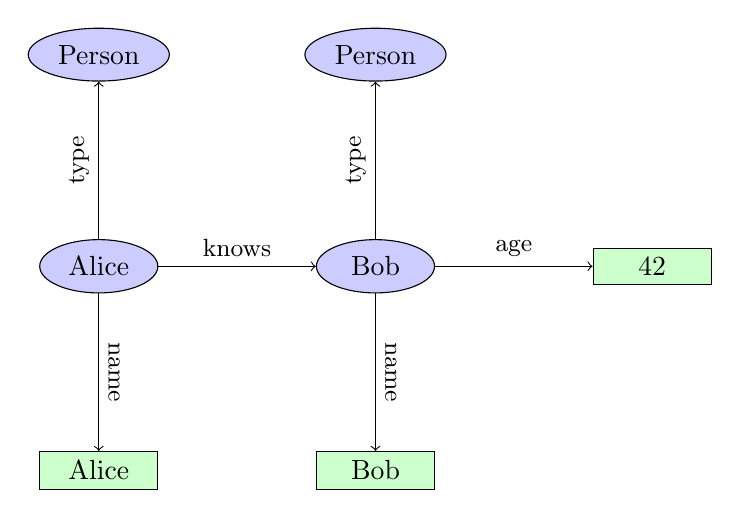
\begin{tikzpicture}[
    node distance=2cm,
    entity/.style={ellipse, draw, fill=blue!20, minimum width=1.5cm, align=center},
    literal/.style={rectangle, draw, fill=green!20, minimum width=1.5cm, align=center},
    property/.style={font=\small, above, sloped}
]

% Nodes
\node[entity] (alice) {Alice};
\node[entity, right=of alice] (bob) {Bob};
\node[literal, below=of alice] (aliceName) {Alice};
\node[literal, below=of bob] (bobName) {Bob};
\node[literal, right=of bob] (bobAge) {42};
\node[entity, above=of alice] (personAlice) {Person};
\node[entity, above=of bob] (personBob) {Person};

% Edges
\draw[->] (alice) -- node[property] {type} (personAlice);
\draw[->] (bob) -- node[property] {type} (personBob);
\draw[->] (alice) -- node[property] {name} (aliceName);
\draw[->] (bob) -- node[property] {name} (bobName);
\draw[->] (alice) -- node[property] {knows} (bob);
\draw[->] (bob) -- node[property] {age} (bobAge);

\end{tikzpicture}
\end{center}

\subsection{N-Triples}
In N-Triples, each line encodes a single triple. IRIs are written enclosed in angle brackets, blank nodes as \texttt{\_:label}, and literals as quoted strings optionally followed by \texttt{\textasciicircum\textasciicircum} and a datatype IRI or by a language tag. Each triple is terminated with a dot. The example graph in N-Triples is:

\begin{lstlisting}[caption=Example graph in N-Triples]
<http://example.org/Alice> <http://www.w3.org/1999/02/22-rdf-syntax-ns#type> <http://xmlns.com/foaf/0.1/Person> .
<http://example.org/Alice> <http://xmlns.com/foaf/0.1/name> "Alice" .
<http://example.org/Alice> <http://xmlns.com/foaf/0.1/knows> <http://example.org/Bob> .
<http://example.org/Bob> <http://www.w3.org/1999/02/22-rdf-syntax-ns#type> <http://xmlns.com/foaf/0.1/Person> .
<http://example.org/Bob> <http://xmlns.com/foaf/0.1/name> "Bob" .
<http://example.org/Bob> <http://xmlns.com/foaf/0.1/age> "42"^^<http://www.w3.org/2001/XMLSchema#integer> .
\end{lstlisting}

N-Triples is very fast and easy to parse, but inefficient in terms of storage space because IRIs are repeated in full for every triple.

\subsection{Turtle}
Turtle extends N-Triples with convenient abbreviations. The \texttt{@prefix} directive declares namespace prefixes, \texttt{@base} sets a base IRI. A semicolon repeats the subject, a comma repeats both subject and predicate. Blank nodes can be written with square brackets containing predicate-object pairs. The example graph in Turtle is:

\begin{lstlisting}[caption=Example graph in Turtle]
@prefix ex: <http://example.org/> .
@prefix foaf: <http://xmlns.com/foaf/0.1/> .

ex:Alice a foaf:Person ;
    foaf:name "Alice" ;
    foaf:knows ex:Bob .

ex:Bob a foaf:Person ;
    foaf:name "Bob" ;
    foaf:age 42 .
\end{lstlisting}

\begin{note}{}
    Note the use of the keyword \texttt{a} as a shorthand for \texttt{rdf:type}, and the fact that \texttt{42} is written without an explicit datatype because Turtle maps plain integer numerals to \texttt{xsd:integer} by default.
\end{note}

\subsection{JSON-LD}
JSON-LD encodes the RDF graph as a JSON object. IRIs are shortened using a \texttt{@context} mapping, subjects are JSON objects identified by their IRI as the key, and properties become keys within those objects. The example graph in JSON-LD is:

\begin{lstlisting}[caption=Example graph in JSON-LD]
{
  "@context": {
    "ex": "http://example.org/",
    "foaf": "http://xmlns.com/foaf/0.1/"
  },
  "@graph": [
    {
      "@id": "ex:Alice",
      "@type": "foaf:Person",
      "foaf:name": "Alice",
      "foaf:knows": { "@id": "ex:Bob" }
    },
    {
      "@id": "ex:Bob",
      "@type": "foaf:Person",
      "foaf:name": "Bob",
      "foaf:age": 42
    }
  ]
}
\end{lstlisting}

\subsection{Other Forms}
RDF/XML is an XML-based syntax that was the original standard for RDF serialization. RDFa (RDF in Attributes) embeds RDF data within HTML attributes, allowing structured data to be integrated directly into Web pages.

\section{RDF Datasets}
An RDF dataset is a collection of RDF graphs, consisting of exactly one default graph and zero or more named graphs identified by an IRI. 
Datasets introduce the notion of grouping triples into separate graphs, which enables several powerful features, such as: 

\begin{itemize}
    \item \emph{Provenance tracking}: Triples can be placed in named graphs that record their origin, such as the source dataset from which they were extracted or the time at which they were added. 

    \item \emph{Data access control:} Different named graphs can represent different visibility scopes, with some graphs being public and others restricted to certain users.
\end{itemize}

In practice, RDF datasets are often stored as quads (subject, predicate, object, graph) rather than triples. 
The fourth element identifies the graph to which the triple belongs. 

The default graph is a special graph that, by convention, contains triples that are not explicitly assigned to any named graph, or it can be configured to contain the union of some or all named graphs. 

\section{Limitations}
Since an RDF triple encodes a binary relationship, representing a relationship of higher arity (e.g., a purchase involving a buyer, seller, object, and price) requires a workaround. The standard approach is \keyword{reification}: introducing a new resource that represents the relationship and attaching the components as separate binary properties of that resource. For example, consider a relational table \texttt{Purchases} with columns \texttt{buyer}, \texttt{seller}, \texttt{item}, and \texttt{price}:

\begin{table}[H]
    \centering
    \begin{tabular}{cccc}
        \toprule
        \textbf{buyer} & \textbf{seller} & \textbf{item} & \textbf{price} \\
        \midrule
        Alice & Bob & Laptop & 1200 \\
        Carol & Dave & Phone & 800 \\
        \bottomrule
    \end{tabular}
\end{table}

Using RDB2RDF (Relational Database to RDF), one defines a mapping that transforms each row into a set of triples. 
Each row becomes a new resource (a blank node or an IRI), and each column becomes a property of that resource. 
The mapping for the \texttt{Purchases} table would produce, for the first row, the following triples in Turtle:

\begin{lstlisting}[caption=RDB2RDF output for a purchase]
@prefix ex: <http://example.org/> .

ex:purchase-1 a ex:Purchase ;
                ex:buyer ex:Alice ;
                ex:seller ex:Bob ;
                ex:item ex:Laptop ;
                ex:price 1200 .
\end{lstlisting}

Here, \texttt{ex:purchase-1} is the new resource introduced to reify the purchase relationship, and the four columns become four separate binary properties. 

Another limitation is that, since the triples in an RDF graph are unordered, representing ordered lists has no single standard solution. Two common approaches are: 

\begin{itemize}
    \item \emph{RDF Collections} model ordered lists as linked list structures using the vocabulary \texttt{rdf:first} and \texttt{rdf:rest}, with \texttt{rdf:nil} terminating the list. The following graph represents the ordered list \texttt{[Alice, Bob, Carol]}:

\begin{lstlisting}[caption={RDF Collection for Alice, Bob, Carol}]
@prefix ex: <http://example.org/> .
@prefix rdf: <http://www.w3.org/1999/02/22-rdf-syntax-ns#> .

ex:list rdf:first ex:Alice ;
        rdf:rest [ rdf:first ex:Bob ;
                   rdf:rest [ rdf:first ex:Carol ;
                              rdf:rest rdf:nil ] ] .
\end{lstlisting}

    Each node in the linked list has a \texttt{rdf:first} property pointing to the element and an \texttt{rdf:rest} property pointing to the remainder of the list. Blank nodes (written with square brackets) represent the intermediate cons cells. This structure allows arbitrary-length lists but can be cumbersome to traverse.

    \item \emph{RDF Containers} represent order using indexed membership properties: \texttt{rdf:\_1}, \texttt{rdf:\_2}, and so on. The same list \texttt{[Alice, Bob, Carol]} as an RDF Container (\texttt{rdf:Seq}) is:

    \begin{lstlisting}[caption={RDF Container for Alice, Bob, Carol}]
@prefix ex: <http://example.org/> .
@prefix rdf: <http://www.w3.org/1999/02/22-rdf-syntax-ns#> .

ex:list rdf:type rdf:Seq ;
        rdf:_1 ex:Alice ;
        rdf:_2 ex:Bob ;
        rdf:_3 ex:Carol .
    \end{lstlisting}

    Containers are more compact than Collections for small lists, but they do not guarantee that the indices form a contiguous sequence.
\end{itemize}

\section{SPARQL}
SPARQL (SPARQL Protocol and RDF Query Language) is the standard query language for RDF graphs, standardized by the W3C. The SPARQL specification consists of several major parts:
\begin{itemize}
    \item A \textbf{query language} for retrieving and manipulating RDF data.
    \item \textbf{Result formats} (e.g., XML, JSON, CSV, TSV) for encoding query results.
    \item An \textbf{update language} (SPARQL Update) for inserting, modifying, and deleting RDF triples.
    \item \textbf{Protocols} for communicating with online SPARQL services (SPARQL Protocol), typically over HTTP.
    \item A \textbf{vocabulary} for describing SPARQL services (SPARQL Service Description).
\end{itemize}

\subsection{Queries}
SPARQL queries use \keyword{variables}, which are marked with an initial \code{?} (or \code{\$}). Variables can appear in the position of subjects, predicates, or objects within \keyword{triple patterns}, and are matched against the corresponding elements in the RDF graph. The syntax of SPARQL closely resembles Turtle (the standard RDF serialization format), making it natural to read and write for those familiar with RDF.

The structure of a SPARQL \code{SELECT} query consists of the following clauses, in order:
\begin{enumerate}
    \item \textbf{Prologue}: An optional sequence of \code{PREFIX} declarations (and optionally \code{BASE}) that define namespace abbreviations used throughout the query, exactly as in Turtle.
    \item \textbf{Select clause} (\code{SELECT}): Specifies which variables to project in the result set. This clause can also include aggregation, expressions (\code{SELECT ?x (COUNT(?y) AS ?count)}), and the \code{DISTINCT} or \code{REDUCED}\footnote{If \code{REDUCED} is specified, the query engine may remove duplicates, but it is not obligated to do so like with \code{DISTINCT}.} modifiers.
    \item \textbf{Where clause} (\code{WHERE}): Contains the graph pattern to be matched against the RDF graph. The body of the \code{WHERE} clause is a \keyword{basic graph pattern} enclosed in braces, potentially combined with other pattern operators (\code{UNION}, \code{OPTIONAL}, \code{FILTER}, etc.).
    \item \textbf{Solution set modifiers}: Optional clauses applied after pattern matching, including \code{ORDER BY}, \code{LIMIT}, \code{OFFSET}, and \code{GROUP BY} (when used with aggregation).
\end{enumerate}

\begin{definition}{Variable}
    A \keyword{variable} is a string that begins with \code{?} (or \code{\$}), where the string can comprise letters, numbers and the underscore symbol. The variable name is the string after the leading symbol.
\end{definition}

\begin{definition}{Triple Pattern}
    A \keyword{triple pattern} is a triple \(\langle s, p, o\rangle\), where \(s\) and \(o\) are arbitrary RDF terms or variables, and \(p\) is an IRI or variable.
\end{definition}

\begin{definition}{Basic Graph Pattern}
    A \keyword{basic graph pattern} (BGP) is a set of juxtaposed triple patterns, interpreted as in conjunction (i.e., all triple patterns must match simultaneously).
\end{definition}

When working with blank nodes (bnodes), one can associate a temporary identifier to a bnode within a query, so that the same bnode can be referenced in multiple triple patterns. This allows the query to track occurrences of that specific bnode across the pattern.
A \keyword{bnode identifier} in a query is written like a variable but with \code{\_:} as the leading marker (e.g., \code{\_:x}) instead of \code{?}, and \textbf{cannot appear in the \code{SELECT} clause}. 
Alternatively, the shorthand \code{[]} can be used for an anonymous (unnamed) blank node that appears only once.

A given bnode identifier can appear only once per query part\footnote{A \q{query part} refers to each syntactically distinct sub-query or group graph pattern; the same bnode identifier may be reused in separate sub-queries, though best practice is to use fresh labels for clarity.}.

Moreover, one can combine multiple BGPs in the same \code{WHERE} clause by juxtaposing \keyword{group graph patterns}.

\begin{definition}{Group Graph Pattern}
    A group graph pattern (GGP) is an arbitrarily complex pattern inside a pair of curly braces \code{\{...\}}.
    It is \emph{arbitrarily} complex because it can contain just triple patterns --- in this case, it becomes a BGP --- as well as entire subqueries (\texttt{SELECT}-\texttt{WHERE}-...) and nested GGPs.
\end{definition}

So, GGPs are more general patterns and a BGP is a trivial GGP.

One can combine multiple GGPs by separating them with commas. The GGPs are combined using the \code{Join} operation, which combines the solutions of two group graph patterns by matching identical bindings for shared variables, producing a new set of solutions that satisfy both patterns simultaneously. It is equivalent to a natural join over the variable mappings.

\subsubsection{Query Results}
\begin{definition}{Solution Mapping}
    A \keyword{solution mapping} \(\mu\) is a partial function\footnote{A function is said \emph{partial} when it does not map every point of the domain, unlike a \emph{total} function which does.} from the set of variable names to the set of RDF terms.
\end{definition}
The function is partial because a given solution mapping typically binds only the variables that appear in the query's \code{WHERE} clause, and not every possible variable name. 
This reflects the fact that a query result provides bindings only for the variables it actually used.

\begin{definition}{Solution}
    Given an RDF graph \(G\) and a BGP \(P\), a solution mapping \(\mu\) is a \keyword{solution} if it is defined exactly on the variables in \(P\) and there exists a mapping \(\sigma\) from blank nodes to RDF terms such that \(\mu(\sigma(P))\subseteq G\), i.e. \(\mu(\sigma(P))\) are terms that exist in \(G\).
    A BGP \(P\) can yield, over the graph \(G\), several solutions that are contained in the \keyword{solution multiset}\footnote{Compared to a set, a multiset allows multiple occurrences of identical elements. This means that, in a multiset, each item is associated with a cardinality.}(denoted \(\text{eval}_G(P)\)), where the cardinality of each solution \(\mu\) equals the number of distinct \(\sigma\) mappings that satisfy the condition.
\end{definition}

\begin{note}{Connection with Logics}
    A solution can be seen as a model \(\mu\) that satisfies the condition expressed in the BGP \(P\) with a mapping \(\sigma\) that maps the blank nodes (equivalent to existentially quantified variables) to terms of the graph \(G\).
\end{note}

\noindent
Now, let's examine an example to better understand the notion of cardinality.

\begin{example}{}
    Let's consider the following graph \(G\) in Turtle syntax:
    \begin{lstlisting}[style=csstyle]
eg:Arrival eg:actorRole eg:aux1, eg:aux2 .
eg:aux1 eg:actor eg:Adams ;
        eg:character "Louise Banks" .
eg:aux2 eg:actor eg:Renner ;
        eg:character "Ian Donnelly" .
eg:Gravity eg:actorRole [
    eg:actor eg:Bullock ;
    eg:character "Ryan Stone"
] .
    \end{lstlisting}

    The BGP \code{?film eg:actorRole []} yields two solutions \(\mu_1, \mu_2\), where \(\mu_1\) binds \code{?film} to \code{eg:Arrival} with \(\#\mu_1 = 2\) --- the blank node in the BGP can be mapped to both \code{eg:aux1} and \code{eg:aux2} to find a matching subgraph ---, and \(\mu_2\) binds \code{?film} to \code{eg:Gravity}, with \(\#\mu_2 = 1\).

    Now, the BGP \code{?film eg:actorRole [ eg:actor ?person]} yields three solutions, each with cardinality one: \{\code{?film} \(\mapsto\) \code{eg:Arrival}, \code{?person} \(\mapsto\) \code{eg:Adams}\}, \{\code{?film} \(\mapsto\) \code{eg:Arrival}, \code{?person} \(\mapsto\) \code{eg:Renner}\}, and \{\code{?film} \(\mapsto\) \code{eg:Gravity}, \code{?person} \(\mapsto\) \code{eg:Bullock}\}.
    This happens because, once we map the blank node to \code{eg:aux1} (resp. \code{eg:aux2}), the property \code{eg:actor} forces a specific binding for \code{?person}, yielding two separate solution mappings that do not depend on any further blank node mapping \(\sigma\).
    
    In general, if the blank node is \q{opaque} (not connected to any variable), multiple \(\sigma\) choices collapse into a single \(\mu\), and the cardinality counts how many distinct ways the blank node could have been assigned. 
    If the blank node's properties are exposed via a variable, different \(\sigma\) choices produce genuinely different \(\mu\) mappings, and each is counted separately with cardinality 1 (assuming no other ambiguity remains). 
\end{example}

Lastly, let's consider \q{ground}\footnote{In logics, a formula is ground when it does not contain variables.} queries, usually called \keyword{boolean queries}. An example of ground query for the previous example is 
\begin{lstlisting}[language=bash]
SELECT *
WHERE eg:Arrival eg:actorRole eg:aux1 .

# output: true
\end{lstlisting}
Such a query can produce only two kinds of solution multiset: \(\text{eval}(P)_G = \set{}\) (false: the pattern did not match) and \(\text{eval}(P)_G = \set{\emptyset}\) (true: the pattern did match, where \(\emptyset\) denotes the empty mapping).

\subsubsection{Other Query Forms}
Beyond the basic \code{SELECT} form, SPARQL provides three additional query forms:

\begin{itemize}
    \item \textbf{ASK}: A boolean query that tests whether a graph pattern has at least one solution. It returns \code{true} or \code{false}, with no variable bindings. This is useful for checking the existence of certain data without retrieving it.
    
    \item \textbf{CONSTRUCT}: Builds and returns a new RDF graph by substituting variables in a template graph pattern with the bindings obtained from the \code{WHERE} clause. This allows transforming or reshaping RDF data. For example, one might convert data from one vocabulary to another by constructing new triples based on existing patterns.
    
    \item \textbf{DESCRIBE}: Returns an RDF graph that \q{describes} the resources matched by the query. The exact form of the description is implementation-dependent: the SPARQL service decides which triples to include to provide a useful description of the identified resources. This form is useful for exploring unknown data or retrieving a concise bounded description of a resource.
\end{itemize}

\subsection{Advanced SPARQL Querying}
Basic SPARQL relies on basic graph patterns, but BGPs are not powerful enough to express complex queries in a succint way. For example, how would one express, using BGPs only, the query \q{find the descendants of J.S. Bach}? 
It would be necessary to express not only direct connections, but also indirect ones.

\begin{definition}{Property Path}
    In an RDF graph \(G\), we can see a path as a sequence of concatenated triple patterns where the object of a triple is the subject of the following one.
    A \keyword{property path} is the sequence of the predicates of a path.
\end{definition}

Let's make an example to better understand this concept.
\begin{example}{}
    Let's consider the following RDF graph in Turtle syntax:
    \begin{lstlisting}
@prefix eg: <http://example.com>

eg:Alice eg:knows eg:Bob
eg:Bob eg:knows eg:Jim
eg:Jim eg:knows eg:Frank
    \end{lstlisting}

    The longest path of this graph is
    \begin{center}
        \code{eg:Alice eg:knows eg:Bob eg:knows eg:Jim eg:knows eg:Frank}
    \end{center}
    and its lenght is \(3\), which is the number of predicates.
    The associated property path is \code{eg:knows -> eg:knows -> eg:knows}.
\end{example}

A \keyword{property path} can be expressed in regex-like form:
\begin{table}[H]
    \centering
    \caption{SPARQL Property Path Syntax}
    \label{tab:property-path}
    \begin{tabular}{@{}c|l|l@{}}
        \toprule
        \textbf{Construct} & \textbf{Syntax} & \textbf{Meaning} \\
        \midrule
        IRI & \code{iri} & The predicate itself (length 1) \\
        Reverse & \code{\textasciicircum pp} & Inverse path (subject and object swapped) \\
        Sequence & \code{pp1 / pp2} & Concatenation of paths \\
        Alternative & \code{pp1 | pp2} & Either path \\
        Zero or more & \code{pp*} & Path repeated 0 or more times \\
        One or more & \code{pp+} & Path repeated 1 or more times \\
        Zero or one & \code{pp?} & Optional path (0 or 1 occurrence) \\
        Negated property set & \code{!(iri1|...|irin)} & Any IRI \emph{not} in the set \\
        Negated inverse set & \code{!(\textasciicircum iri1|...|\textasciicircum irin)} & Any IRI whose inverse is \emph{not} in the set \\
        \bottomrule
    \end{tabular}
\end{table}
\begin{note}{}
    The precedence between operators is \code{!} \(\succ\) \code{*/+/?} \(\succ\) \code{\textasciicircum} \(\succ\) \code{/} \(\succ\) \code{|}. Negated property sets must always be enclosed in parentheses.
\end{note}

\begin{definition}{Property Path Pattern}
    A \keyword{property path pattern} is a triple \(\langle s, p, o\rangle\), where \(s\) and \(o\) are arbitrary RDF terms and \(p\) is a property path.
\end{definition}

\noindent
A property path pattern is an extension of the triple pattern to property paths instead of basic predicates.
As for triple patterns, the described syntax is purely abstract: we need a way to practically represent it.
This is done by extending the Turtle syntax, allowing property paths to take place of predicates.

\begin{definition}{\(\Path{}\)}
    For a property path \(PP\), the set \(\Path{PP}\) is 
    \[
    \Path{PP} = \begin{cases}
        \{\text{iri}\} & PP=\text{iri}  \\[4pt]
        \bigcup_{i \geq 0}PP^i & PP=PP^* \\[4pt]
        \bigcup_{i \geq 1}PP^i & PP=PP^+ \\[4pt]
        \Path{PP} \cup \{\varepsilon\} & PP=PP? \\[4pt]
        \Reversed{PP} & PP=\text{\textasciicircum}PP \\[4pt]
        \Path{PP_1} \circ \Path{PP_2} & PP=PP_1/PP_2 \\[4pt]
        \Path{PP_1} \cup \Path{PP_2} & PP=PP_1|PP_2 \\[4pt]
        \Path{PP} \setminus \bigcup_{i=1}^{n}\Path{\text{iri}_i} & PP=!(\text{iri}_1|\ldots |\text{iri}_n) \\[4pt]
        \Path{PP} \setminus \bigcup_{i=1}^{n}\Reversed{\Path{\text{iri}_i}} & PP=!(\text{\textasciicircum iri}_1|\ldots | \text{\textasciicircum iri}_n)
    \end{cases}
    \]

    where the following language operations are assumed:
    \begin{align*}
        L_1 \circ L_2 &= \{w_1w_2 : w_1 \in L_1, w_2 \in L_2\} \\
        L^0 &= \{\varepsilon\} \\
        L^{i+1} &= L^{i} \circ L \\
        L^* &= \bigcup_{i \geq 0}L^i
    \end{align*}

    and \(\Reversed{PP}\) makes \(PP\) reversed.  
\end{definition}
Now, we can define a solution for a property path pattern.

\begin{definition}{Solution for a Property Path Pattern}
    Given an RDF graph \(G\) and a property path pattern \(P=\langle s, pp, o \rangle\), a solution mapping \(\mu\) is a solution if and only if there is a bnode mapping \(\sigma\) s.t. \(G\) contains a property path from \(\mu(\sigma(s))\) to \(\mu(\sigma(o))\) containing only predicates in \(\Path{pp}\).
\end{definition}
Moreover, empty paths (\(\varepsilon\)) exist from any node to itself.

Now, we have to explain a bit on how solutions are found by the query engine, so that we will understand some of its unintuitive features.
The official SPARQL 1.1~\cite{sparql11} algebra says that property paths built with \code{*}, \code{+}, \code{?} are evaluated via an ALP (Arbitrary Length Path) algorithm, which is essentially a graph-reachability search. So, ALP searches if a path from \(s\) to \(o\) exists and does not search for all possible paths between these two nodes. 
So, a query containing a property path pattern that comprises \code{*}, \code{+}, \code{?} will yield, if found, a single solution.
On the other hand, property paths that are built only with operators that don't involve unbounded repetition (\code{iri}, \code{\textasciicircum}, \code{/}, \code{|}, \code{!}) are evaluated by composing simple triple patterns with unions and joins between the intermediate solution multisets.

\begin{example}{}
    Consider the following RDF graph in Turtle syntax, describing two independent chains of \code{eg:knows} relations connecting \code{eg:Alice} to \code{eg:Dave}:
    \begin{lstlisting}
@prefix eg: <http://example.com/>

eg:Alice eg:knows eg:Bob , eg:Carol .
eg:Bob   eg:knows eg:Dave .
eg:Carol eg:knows eg:Dave .
    \end{lstlisting}
    There are exactly two distinct paths of length \(2\) from \code{eg:Alice} to \code{eg:Dave}: one through \code{eg:Bob} and one through \code{eg:Carol}.

    Let's evaluate two different, but semantically related, property path patterns against this graph.

    \textbf{Query A: using \(+\) (ALP evaluation)}
    \begin{lstlisting}
SELECT ?o WHERE {
    eg:Alice eg:knows+ ?o .
}
    \end{lstlisting}
    Since \code{+} triggers the ALP algorithm, the engine only checks \emph{reachability} of \code{?o} from \code{eg:Alice} via one or more \code{eg:knows} edges. Even though \code{eg:Dave} is reachable via \emph{two} distinct paths, it is recorded as reachable \emph{once}. The result set is
    \[
        \{\mu_1(?o)=\text{eg:Bob}, \mu_2(?o)=\text{eg:Carol}, \mu_3(?o)=\text{eg:Dave}\}
    \]
    with \(\mu_3\) appearing only once, regardless of how many ways there are to reach \code{eg:Dave}.

    \textbf{Query B: using \(/\) (Join evaluation).}
    \begin{lstlisting}
SELECT ?o WHERE {
    eg:Alice eg:knows/eg:knows ?o .
}
    \end{lstlisting}
    Here \code{eg:knows/eg:knows} is evaluated as
    \[
        \text{Join}\big(\text{eval}(\text{eg:Alice}, \text{eg:knows}, ?v),\ \text{eval}(?v, \text{eg:knows}, ?o)\big),
    \]
    that is a join over the intermediate variable \code{?v}. Since \code{?v} can bind to both \code{eg:Bob} and \code{eg:Carol}, and both lead to \code{eg:Dave}, the join produces \emph{two} solution mappings that agree on \code{?o}:
    \[
        \{\mu_1(?o)=\text{eg:Dave}, \mu_2(?o)=\text{eg:Dave}\}.
    \]
\end{example}

\subsection{Query Modifiers}
Now that we have largely talked about the patterns inside the \code{WHERE} clause, let's focus on other clauses that can be used in a SPARQL query. 
Let's start with the projection clause i.e. (\code{SELECT}).

\subsubsection{\code{SELECT} Clause}
\begin{definition}{Projection of a Solution Mapping}
    Given a solution mapping \(\mu\), we define its \keyword{projection} \(\pi=\mu|_{V}\) as its restriction to \(V\), that is a set of variables.
    The cardinality of \(\pi\) inside the new solution multiset \(\Pi\) is the sum of cardinalities of all \(\nu\in\Omega\) s.t. \(\nu|_{V}=\pi\), where \(\Omega\) is the staring solution multiset.
    In other words, if some \(\nu\in\Omega\) share the same bindings for the variables in \(V\), then their projections \(\nu|_{V}\) collapse in a single solution \(\pi\in\Pi\) and the cardinality of \(\pi\) equals the sum of the cardinalities of the collapsed \(\nu\in\Omega\). 
\end{definition}

\noindent
To make all the solutions of a solution multiset have cardinality one, we have to use the \code{DISTINCT} modifier of the \code{SELECT} clause (i.e., \code{SELECT DISTINCT}).

\subsubsection{Solution Multiset Modifiers}
After the \code{WHERE} clause, SPARQL provides several modifiers to shape the final result set:

\begin{itemize}
    \item \code{ORDER BY}: Sorts the solution sequences according to the value of one or more expressions. The sort order can be ascending (\code{ASC()}) or descending (\code{DESC()}). If neither is specified, ascending order is the default. For example, \code{ORDER BY DESC(...)}.
    
    \item \code{LIMIT}: Restricts the number of solutions returned to at most the specified integer value. For example, \code{LIMIT 10} returns at most 10 solutions. Note that \code{LIMIT} is applied after \code{ORDER BY}, so it is typically used to obtain \q{top-\(k\)} results.
    
    \item \code{OFFSET}: Causes the solutions generated to start after the specified number of solutions. This is useful for pagination when combined with \code{LIMIT} and \code{ORDER BY} (the latter ensures deterministic ordering, which is otherwise not guaranteed by the SPARQL specification).
\end{itemize}

The order of application of these modifiers is fixed: first \code{ORDER BY}, then \code{OFFSET}, then \code{LIMIT}.

\subsubsection{Grouping and Aggregate Functions}
The \code{GROUP BY} clause partitions the solution sequence into groups based on the values of specified expressions. After grouping, aggregate functions can be applied to each group to compute a single representative value. Common aggregate functions include:

\begin{itemize}
    \item \code{COUNT(* | ?var | DISTINCT ?var)}: Counts the number of solutions (or distinct values) in the group.
    \item \code{SUM(?var)}: Computes the numeric sum of the values of \code{?var} over the group.
    \item \code{MIN(?var)} / \code{MAX(?var)}: Returns the minimum or maximum value of \code{?var} in the group.
    \item \code{AVG(?var)}: Computes the arithmetic mean of \code{?var} over the group.
    \item \code{GROUP\_CONCAT(?var; separator="...")}: Concatenates the string values of \code{?var} within the group, using an optional separator.
    \item \code{SAMPLE(?var)}: Returns an arbitrary value of \code{?var} from the group (useful when any representative value suffices).
\end{itemize}

When using \code{GROUP BY}, variables not appearing in the \code{GROUP BY} clause can only be used in the \code{SELECT} clause if they appear inside an aggregate function. If no \code{GROUP BY} is specified but aggregate functions are present in the \code{SELECT} clause, the entire solution sequence is treated as a single implicit group.

\subsubsection{\code{HAVING} Clause}
The \code{HAVING} clause is used to filter groups of solutions based on the values of aggregate functions. It is evaluated \emph{after} the \code{GROUP BY} clause and allows to retain only those groups that satisfy a given condition involving aggregates (e.g., \code{HAVING(COUNT(?x) > 5)}). This is different from the \code{FILTER} clause, which operates on individual solutions \emph{before} grouping and cannot reference aggregates.

\subsubsection{\code{FILTER} Clause}
The \code{FILTER} clause is used inside the \code{WHERE} clause to express conditions that restrict solutions based on computed values, rather than on the RDF graph structure (and hence are not expressible as simple triple patterns). Filters operate on the solution multiset by discarding those solutions for which the filter condition evaluates to \code{false} or raises an error; they cannot introduce new solutions.

A \code{FILTER} applies to all variables introduced in the group graph pattern in which it appears. Its scope is the entire pattern, not just the immediately preceding triple pattern.
    
Filters make sense only when applied to variables that have already been bound earlier in the \code{WHERE} clause.

\begin{note}{}
    The query engine is free to reorder filters (and other operations) for optimization, provided the overall evaluation remains logically equivalent to the original query.
\end{note}

Filter expressions can include boolean operators (\code{!}, \code{\&\&}, \code{||}), comparisons (\code{=}, \code{!=}, \code{<}, \code{>}, \code{<=}, \code{>=}), arithmetic, and built-in functions such as \code{isIRI()}, \code{isBlank()}, \code{isLiteral()}, \code{bound()}, \code{str()}, \code{lang()}, \code{regex()}, \code{strstarts()}, \code{strends()}, \code{contains()}, and others.

However, many filters and functions only make sense for certain types of terms (e.g., \code{year} can be applied to \code{date}s only).
When a filter is applied to an incompatible type, an \emph{error} is typically returned. 
We will later explain how errors are handled in SPARQL.

\subsubsection{\code{UNION}}

The \code{UNION} operator combines the solution multisets produced by two group graph patterns. 
Given two patterns \(P_1\) and \(P_2\), the expression \code{\{ P1 \} UNION \{ P2 \}} returns every solution that matches \(P_1\) \emph{or} \(P_2\) (or both). 
The multiplicity of each solution in the result is the \textbf{sum} of its multiplicities in the two input multisets: if a solution appears \(m\) times in the result of \(P_1\) and \(n\) times in the result of \(P_2\), it appears \(m + n\) times in the union.

\code{UNION} can be combined with \code{DISTINCT} to eliminate duplicates, producing a set rather than a multiset. 
For example:
\begin{lstlisting}[language=SQL, caption={UNION with DISTINCT}]
SELECT DISTINCT ?person WHERE {
  { ?person :hasParent :Alice }
  UNION
  { ?person :hasParent :Bob }
}
\end{lstlisting}
This returns each person who has either \code{:Alice} or \code{:Bob} as a parent, without duplicates.

\code{UNION} is processed independently of surrounding patterns, but the combined result must still satisfy any outer patterns and filters.

\subsubsection{\code{MINUS}}

The \code{MINUS} operator computes the set difference between two solution multisets. 
Given two patterns \(P_1\) and \(P_2\), the expression \code{\{ P1 \} MINUS \{ P2 \}} returns the solutions for \(P_1\) that are not solutions for \(P_2\).

The multiplicity of each retained solution equals its multiplicity in \(P_1\).

\begin{note}{MINUS vs. FILTER NOT EXISTS}
    Similar results can often be achieved with \code{FILTER NOT EXISTS}, but the two behave differently. For example, consider two GGPs, \code{P1} and \code{P2}, that do \emph{not} share any variables.
    Now,
    \begin{itemize}
        \item \code{\{ P1 \} MINUS \{ P2 \}} contains \emph{all} solutions of \(P_1\).
        \item \code{FILTER NOT EXISTS \{ P2 \}}: \code{NOT EXISTS} evaluates to \code{false} if \(P_2\) has \emph{at least} a solution, regardless of variable compatibility with \(P_1\). In this case, the filter removes \emph{all} outer solutions.
    \end{itemize}
    In general, \code{MINUS} operates on \emph{solution compatibility}, while \code{FILTER NOT EXISTS} checks \emph{pattern existence} in the dataset, taking into account variable substitutions from the outer scope.
\end{note}

\subsubsection{\code{OPTIONAL}}

The \code{OPTIONAL} operator allows a GGP to be matched \emph{if possible}, without eliminating solutions when the pattern fails. 
Given two patterns \(P_1\) and \(P_2\), the expression \code{\{ P1 \} OPTIONAL \{ P2 \}} yields a solution \(\mu\) s.t. 
\begin{itemize}
    \item \(\mu\) is a solution for \(P_1\)
    \item if \(\mu\) is not a solution for \(P_2\), the variables that appear only in \(P_2\) are left unbound.
\end{itemize}
This is analogous to a \emph{left outer join} in SQL: all results from the mandatory (left) pattern are kept, and optional (right) pattern information is attached where available.

\begin{example}{OPTIONAL Pattern}
    Retrieve all persons and, if available, their email addresses:
    \begin{lstlisting}[language=SQL, caption={Using OPTIONAL for missing data}]
SELECT ?person ?email WHERE {
    ?person rdf:type :Person .
    OPTIONAL { ?person :hasEmail ?email }
}
    \end{lstlisting}
    Persons without an email are still returned, with \code{?email} unbound.
\end{example}

Multiple \code{OPTIONAL} clauses are evaluated sequentially: each optional pattern can use variables bound in mandatory patterns or in preceding optional patterns that successfully matched.

\subsubsection{Subqueries}

Subqueries allow the results of one query to be used as part of another. A subquery is enclosed in curly braces and behaves as a complete \code{SELECT} query within a larger query. 
It returns a solution multiset, and the outer query operates over these results exactly as it would over triple patterns.
A subquery is evaluated independently, producing a multiset of solutions over its projected variables.

Order is not preserved from the inner query to the outer query, as solution multisets carry no ordering information, unless \code{ORDER BY} is used, as in standard queries.

Variables projected by the subquery can be used in the outer query. Variables used only internally to the subquery are not visible outside.

\begin{example}{}
    Find all persons who have authored more than five papers, along with their total count:
    \begin{lstlisting}[language=SQL, caption={Subquery for pre-aggregation}]
SELECT ?person ?paperCount WHERE {
    {
        SELECT ?person (COUNT(?paper) AS ?paperCount) WHERE {
            ?person :authored ?paper .
        }
        GROUP BY ?person
    }
    FILTER(?paperCount > 5)
}
    \end{lstlisting}
    The inner subquery computes the paper count per person, and the outer query filters on that count.
\end{example}

Instead of running a subquery, which can be costly, it is sometimes possible to inject solution multisets (as a subquery would produce) directly into the query evaluation using \code{VALUES} and \code{BIND}.

\subsubsection{\code{VALUES}}
The injected solution multiset is \emph{constant} (contains only IRIs and literals). 

\begin{example}{}
    We want to find all the people who know Alice, who are a composer and who have a child.
    \begin{lstlisting}[language=SQL]
SELECT DISTINCT ?sub WHERE {
    VALUES (?predicate ?obj) {
        (eg:knows eg:Alice)
        (eg:profession eg:Composer)
        (eg:hasChild UNDEF)
    }
    ?sub ?predicate ?obj
}
    \end{lstlisting}
    Each row provides bindings for the specified variables. The special value \keyword{\code{UNDEF}} leaves a variable unbound for that row, meaning the query engine should treat it as a free variable to be matched against the data.
\end{example}

\subsubsection{\code{BIND}}

\code{BIND} allows to bind a variable with a constant or \emph{computed} value inside the query evaluation.

\begin{example}{}
    We want to find the people who have their birth year as their favourite number. 
    \begin{lstlisting}[language=SQL]
SELECT DISTINCT ?sub WHERE {
    ?sub eg:dob ?date .
    BIND (YEAR(?date) AS ?year)
    ?sub eg:favourite_number ?year
}
    \end{lstlisting}
    This could have been also done with a \code{FILTER} statement, but this way is more direct.
\end{example}

\begin{note}{}
    Note that not only is \code{BIND} equivalent to expression assignments with \code{AS} in \code{SELECT} (e.g., \code{SELECT (expr AS ?var)}), but variables bound via \code{BIND} can be used \emph{inside} the group graph pattern as soon as they have been bound---in later triple patterns, filters, or subsequent \code{BIND} expressions within the same scope. 
    This is a significant advantage when the computed value needs to participate in pattern matching.

    Assignments of \textbf{constants} to variables are better realized with \code{VALUES}, which can be placed before or after other patterns using the variable. Because \code{VALUES} provides a static data table, the query engine can optimize it more aggressively than a \code{BIND} with a constant expression.
\end{note}

\subsection{Errors in SPARQL}

SPARQL follows a specific error handling philosophy based on the concept of \keyword{Effective Boolean Value} (EBV). 
Rather than halting query execution on type errors, SPARQL propagates errors through the evaluation process according to defined rules.

\begin{definition}{Effective Boolean Value (EBV)}
    The \keyword{Effective Boolean Value} of a term is defined as follows:
    \begin{itemize}
        \item The EBV of \textbf{true} is \code{true}.
        \item The EBV of \textbf{false} is \code{false}.
        \item The EBV of a \textbf{literal} with datatype \code{xsd:boolean} is the corresponding boolean value.
        \item The EBV of a \textbf{string} literal (\code{xsd:string} or plain literal with no language tag) is \code{false} if the string is empty, and \code{true} otherwise.
        \item The EBV of a \textbf{numeric} literal is \code{false} if the value is zero or \code{NaN}, and \code{true} otherwise.
        \item The EBV of \textbf{any other term} (including unbound variables, blank nodes, IRIs, and literals of other datatypes) is a \textbf{type error}.
    \end{itemize}
\end{definition}

\subsubsection{Error Propagation}
Error propagation in SPARQL works as follows:
\begin{itemize}
    \item When a filter or function encounters a type error (e.g., applying \code{year()} to a string), it produces an \textbf{error}, not a value.
    \item In logical expressions, errors are treated according to a \textbf{three-valued logic}:
    \begin{itemize}
        \item \code{true AND error} \(\to\) \textbf{error}
        \item \code{false AND error} \(\to\) \textbf{false} (short-circuit evaluation: the conjunction cannot become true)
        \item \code{true OR error} \(\to\) \textbf{true} (short-circuit: the disjunction is already true)
        \item \code{false OR error} \(\to\) \textbf{error}
        \item \code{NOT error} \(\to\) \textbf{error}
    \end{itemize}
    \item In a \code{FILTER} clause, if the overall filter expression evaluates to \textbf{true}, the solution is kept; if it evaluates to \textbf{false} or \textbf{error}, the solution is \textbf{discarded}. Errors thus behave like \code{false} for filtering purposes, but with different propagation behavior inside compound expressions.
\end{itemize}

This design ensures that a type error on a single tuple does not abort the entire query: only the offending solution is filtered out, while valid solutions are still returned. 
This is analogous to how SQL's \code{NULL} propagation works in \code{WHERE} clauses, but with explicit three-valued logic for error handling.

\subsection{Some SPARQL Queries Examples}
Now that we have all the required notions, let's see some examples of SPARQL queries on a example RDF graph.
Let's consider the following graph represented in Turtle syntax:
\begin{lstlisting}
# Prefixes
@prefix uni: <http://example.org/university#> .
@prefix foaf: <http://xmlns.com/foaf/0.1/> .
@prefix rdfs: <http://www.w3.org/2000/01/rdf-schema#> .
@prefix rdf: <http://www.w3.org/1999/02/22-rdf-syntax-ns#> .
@prefix xsd: <http://www.w3.org/2001/XMLSchema#> .

# Ontology: Classes with hierarchy
foaf:Person a rdfs:Class ;
    rdfs:label "Person" .

uni:Student a rdfs:Class ;
    rdfs:subClassOf foaf:Person ;
    rdfs:label "Student" .

uni:Teacher a rdfs:Class ;
    rdfs:subClassOf foaf:Person ;
    rdfs:label "Teacher" .

uni:Course a rdfs:Class ;
    rdfs:label "Course" .

uni:Exam a rdfs:Class ;
    rdfs:label "Exam" .

# RDF Graph

# Generic persons (neither students nor teachers)
uni:secretary a foaf:Person ;
    foaf:name "Gennaro Locascio" .

# Teachers
uni:prof_rossi a uni:Teacher ;
    foaf:name "Mario Rossi" .

# Students
uni:anna a uni:Student ;
    foaf:name "Anna Verdi" .

uni:luca a uni:Student ;
    foaf:name "Luca Bianchi" .

# Courses
uni:computer_science a uni:Course ;
    foaf:name "Computer Science" ;
    uni:credits 6 .

uni:mathematics a uni:Course ;
    foaf:name "Mathematics" ;
    uni:credits 9 .

# Exams (exam instances with grades)
uni:exam1 a uni:Exam ;
    uni:grade 28 ;
    uni:examForCourse uni:computer_science .

uni:exam2 a uni:Exam ;
    uni:grade 30 ;
    uni:examForCourse uni:mathematics .

uni:exam3 a uni:Exam ;
    uni:grade 25 ;
    uni:examForCourse uni:computer_science .

# Relationships
uni:prof_rossi uni:teaches uni:computer_science, uni:mathematics .
uni:anna uni:enrolledIn uni:mathematics .
uni:luca uni:enrolledIn uni:computer_science .
uni:anna uni:hasExam uni:exam1, uni:exam2 .
uni:luca uni:hasExam uni:exam3 .
\end{lstlisting}

Here are some examples of SPARQL requests based on the graph above, along with their respective queries and a brief explanation of the critical design choices.

\subsubsection*{Example 1: Counting Enrolled Students per Course}
\textbf{Request:} Find all courses and for each of them the number of enrolled students.

\begin{lstlisting}
SELECT ?c (COUNT(?s) AS ?enrolled)
WHERE {
    {
        SELECT ?c
        WHERE {
            ?c a uni:Course .
        }
    }
    OPTIONAL {  
        ?s a uni:Student;
           uni:enrolledIn ?c .
    }
}
GROUP BY ?c
\end{lstlisting}
\textbf{Critical Choices:} 
The use of \texttt{OPTIONAL} is crucial here. If we used a standard graph pattern, courses with zero enrolled students would be completely excluded from the results. By isolating the courses in a subquery and making the student enrollment optional, we ensure all courses are listed, returning a count of 0 for empty courses. The \texttt{GROUP BY} clause is mandatory since we are mixing an aggregate function (\texttt{COUNT}) with a standard projected variable (\texttt{?c}).

\subsubsection*{Example 2: Filtering on Specific Paths}
\textbf{Request:} Find all students who have taken at least one exam for a course taught by Prof. Mario Rossi with a grade higher than 26.

\begin{lstlisting}
SELECT DISTINCT ?s
WHERE {
    {
        SELECT ?c
        WHERE {
            uni:prof_rossi uni:teaches ?c .
        }
    }
    ?s uni:hasExam ?e .
    ?e uni:examForCourse ?c .
    ?e uni:grade ?g .
    FILTER (?g > 26)
}
\end{lstlisting}
\textbf{Critical Choices:} 
\texttt{SELECT DISTINCT} prevents duplicate rows. Without it, a student who passed multiple exams with Prof. Rossi (both $> 26$) would appear multiple times in the results. The \texttt{FILTER} clause must enclose its condition in parentheses.

\subsubsection*{Example 3: Handling Missing Data}
\textbf{Request:} Find all persons with their names and, if they have it, the degree course they are enrolled in.

\begin{lstlisting}
SELECT ?p ?pname ?dc
WHERE {
    ?p a foaf:Person ;
       foaf:name ?pname .
    OPTIONAL {
        ?p uni:enrolledIn ?dc .
    }
}
\end{lstlisting}
\textbf{Critical Choices:} 
Since the \texttt{foaf:Person} class includes teachers and secretaries who are not enrolled in any course, the \texttt{OPTIONAL} block is necessary. This guarantees that all persons are returned; the \texttt{?dc} variable will simply be unbound (empty) for non-student persons.

\subsubsection*{Example 4: Global Aggregation via Subqueries}
\textbf{Request:} Find all students who have taken at least one exam with a grade higher than the general average of all exams (taken by all students).

\begin{lstlisting}
SELECT DISTINCT ?s
WHERE {
    {
        SELECT (AVG(?g) AS ?average)
        WHERE {
            ?e a uni:Exam ;
               uni:grade ?g .
        }
    }
    ?s uni:hasExam ?e .
    ?e uni:grade ?g .
    FILTER (?g > ?average)
}
\end{lstlisting}
\textbf{Critical Choices:} 
The subquery effectively computes a single, global aggregate value (\texttt{?average}) and projects it into the outer scope. SPARQL 1.1 scoping rules allow variables like \texttt{?e} and \texttt{?g} to be reused safely inside and outside the subquery because the subquery only projects \texttt{?average}, preventing namespace collisions.

\section{An example of RDF Knowledge Graph: Wikidata}
Wikidata is Wikipedia's knowledge graph. Its practical applications stem from its role as a central, structured data hub: it provides data for Wikipedia infoboxes across all languages, powers the Google Knowledge Graph, and enables complex cross-domain queries, making it a fundamental resource for research, data integration, and AI systems.

Wikidata can be seen as a:
\begin{itemize}
    \item \emph{Document-centric knowledge base}: Data are grouped by pages, where a page represents the subject of triples. Each page contains all statements about that subject, along with its labels, aliases, and site links. This organization makes editing and maintenance straightforward for contributors.
    \item \emph{Graph-structured knowledge base}: Data can be viewed as a giant, interconnected RDF graph where entities are nodes and properties are edges, enabling expressive queries and knowledge discovery across domains.
\end{itemize}

\begin{definition}{Wikidata Entity Document}
    A Wikidata \keyword{entity document} is an object with:
    \begin{itemize}
        \item \emph{Entity ID}: a language-independent id (e.g. \code{Q17515} identifies Diego Armando Maradona);
        \item \emph{Terms header}: a list of language-specific aliases (e.g. \q{El Pibe de Oro} for Italian);
        \item \emph{Statements}: an unordered set of statements, which are subject-property-value triples representing properties that the entity has. Each statement can have \emph{qualifiers}, which are property-value couples that add further information about it, and \emph{references} --- one or more sources about it. 
            A statement has a rank (normal, preferred, deprecated) to encode its significance\footnote{Preferred statements are marked as the most important; deprecated ones are known to be wrong but kept for reference.}. 
            For example, D.A. Maradona has the statement \code{Q17515} \(\to\) \q{member of sports team} \(\to\) \q{SSC Napoli} with qualifier (it is not the only one) \code{start time}\(\to\) \code{1984};
        \item \emph{Site links}: connections to pages on other Wikimedia projects realise entity-level information integration.
    \end{itemize}
\end{definition}

\subsection{From Wikidata to RDF}
Wikidata is internally stored in JSON, which is a document-centric format, and so data has to be converted to RDF to allow SPARQL queries.
Before converting Wikidata to the RDF format, some discrepancies between the two must be resolved:
\begin{enumerate}
    \item Wikidata statements have qualifiers, property-value pairs that add information to the statement;
    \item Wikidata property types do not correspond to XML Schema types; 
    \item Wikidata IDs are not immediately IRIs.
\end{enumerate}
Apart from these differences, Wikidata and RDF are very similar: 
\begin{enumerate}
    \item Both are directed labeled graphs;
    \item All data that appear inside a statement can be subjects/objects in other statements: Wikidata is self-explaining. 
    \item The order of statements does not matter.
\end{enumerate}

To represent qualifiers, we reify the overall statement into a standalone entity and then connect it to the annotations by creating a triple for each annotation as object and the overall statement as subject.
Moreover, the annotation properties with \q{preferred} rank become objects of direct subject-property-object, to allow a more direct navigation for relevant information.
If no \q{preferred} annotation properties exist, those with \q{normal} rank will take their place, while \q{deprecated} ones cannot.

In general, each Wikidata property turns into several RDF properties, whose types are defined by a \keyword{namespace} mechanism.
\begin{table}[H]
    \centering
    \caption{Wikidata RDF namespaces}
    \label{tab:wikidata-namespaces}
    \begin{tabular}{@{}llp{5cm}@{}}
        \hline
        \textbf{Prefix} & \textbf{Namespace URI} & \textbf{Example} \\
        \hline
        \texttt{wd:} & \texttt{http://www.wikidata.org/entity/} & \texttt{wd:Q17515} (Maradona) \\
        \texttt{wdt:} & \texttt{http://www.wikidata.org/prop/direct/} & \texttt{wdt:P54} (member of sports team) \\
        \texttt{p:} & \texttt{http://www.wikidata.org/prop/} & \texttt{p:P54} (statement node) \\
        \texttt{ps:} & \texttt{http://www.wikidata.org/prop/statement/} & \texttt{ps:P54} (statement value) \\
        \texttt{pq:} & \texttt{http://www.wikidata.org/prop/qualifier/} & \texttt{pq:P580} (start time qualifier) \\
        \texttt{pr:} & \texttt{http://www.wikidata.org/prop/reference/} & \texttt{pr:P248} (stated in reference) \\
        \texttt{wdno:} & \texttt{http://www.wikidata.org/prop/novalue/} & \texttt{wdno:P40} (no children) \\
        \texttt{wds:} & \texttt{http://www.wikidata.org/entity/statement/} & \texttt{wds:Q17515-...} (statement ID) \\
        \texttt{wdref:} & \texttt{http://www.wikidata.org/reference/} & \texttt{wdref:...} (reference ID) \\
        \texttt{wikibase:} & \texttt{http://wikiba.se/ontology\#} & \texttt{wikibase:rank} (links, for example, with \texttt{wikibase:NormalRank}) \\
        \hline
    \end{tabular}
\end{table}

\noindent
Finally, all IDs, property types, values (and complex values) are transformed into proper IRIs. For example, the entity ID \code{Q17515} becomes the IRI 
\begin{center}
    \code{http://www.wikidata.org/entity/Q17515}
\end{center}
while the property \code{P54} (member of sports team) becomes the direct property IRI 
\begin{center}
    \code{http://www.wikidata.org/prop/direct/P54} 
\end{center}
for simple truthy statements, and the statement-level property IRI 
\begin{center}
    \code{http://www.wikidata.org/prop/P54} 
\end{center}
when reified statements with qualifiers or references are needed.

\begin{example}{}
    The previously mentioned statement about D.A. Maradona is transformed in the following RDF Turtle code:
    \begin{lstlisting}
# The direct statement
# (Maradona) (direct: member of sports team) (SSC Napoli)
wd:Q17515 wdt:P54 wd:Q128326 . 

# The reified statement
# (Maradona) (has statement: member of sports team) (Statement ID)
wd:Q17515 p:P54 wds:Q17515-38b4d8ec-4f81-5a63-a20c-7b06606a247e .

# (Statement ID) (statement value: member of sports team) (SSC Napoli)
wds:Q17515-38b4d8ec-4f81-5a63-a20c-7b06606a247e ps:P54 wd:Q128326 .

# (Statement ID) (qualifier: start time) (1984)
wds:Q17515-38b4d8ec-4f81-5a63-a20c-7b06606a247e pq:P580 "1984-01-01T00:00:00Z"^^xsd:dateTime .
    \end{lstlisting}
\end{example}

\subsection{Wikidata SPARQL Query Service (WDQS)}
The Wikidata Query Service (WDQS) is a public SPARQL endpoint that provides live, low-latency access to Wikidata's RDF data, updated in sync with edits made to Wikidata. It allows users to run complex queries over the entire knowledge graph without any local setup.
Common ways to access WDQS include:
\begin{itemize}
    \item \emph{Web Interface}: The primary access point is the web-based query editor at \url{https://query.wikidata.org/}, which features syntax highlighting, autocompletion, and graphical result visualization tools.
    \item \emph{SPARQL Endpoint}: Direct programmatic access via HTTP requests to the endpoint \url{https://query.wikidata.org/sparql}, supporting both GET and POST methods for integrating Wikidata queries into applications and scripts.
    \item \emph{Client Libraries}: Various programming language libraries (such as \texttt{SPARQLWrapper} for Python) provide convenient wrappers around the endpoint, simplifying query execution and result handling in code.
\end{itemize}

\begin{example}{}
    Navigate to \url{https://query.wikidata.org/} and type the following SPARQL query to find all the players who have played with D.~A.~Maradona. You should find 480 results.
    \begin{lstlisting}[language=sql]
PREFIX wd: <http://www.wikidata.org/entity/>
PREFIX wdt: <http://www.wikidata.org/prop/direct/>
PREFIX rdfs: <http://www.w3.org/2000/01/rdf-schema#>

SELECT ?playerLabel ?clubLabel 
WHERE {
    wd:Q17515 p:P54 ?stmtM . # P54 is the 'member of sports team' property id.
    ?stmtM ps:P54 ?club .
    ?stmtM pq:P580 ?startYearM ;
          pq:P582 ?endYearM .

    ?player wdt:P106 wd:Q937857 . # P106 is the 'occupation' property id; Q937857 is the id of 'association football player'.
    FILTER(?player != wd:Q17515) # we filter out Maradona himself
    ?player p:P54 ?stmt .
    ?stmt ps:P54 ?club .
    ?stmt pq:P580 ?startYear ;
           pq:P582 ?endYear .
    FILTER(?startYearM <= ?endYear && ?endYearM >= ?startYear)
    
    ?player rdfs:label ?playerLabel .
    FILTER(LANG(?playerLabel) = "en")
    ?club rdfs:label ?clubLabel .
    FILTER(LANG(?clubLabel) = "en")
}
ORDER BY ?clubLabel ?playerLabel
    \end{lstlisting}
\end{example}


\whitepage{}
\printbibliography
\makebackcover{}

\end{document}